\RequirePackage{etex}
\documentclass{pas}

%=================================================================
% Idioma y citas
%=================================================================
\usepackage[spanish]{babel}
\usepackage[authoryear]{natbib}

%=================================================================
% Figuras y gráficos
%=================================================================
\usepackage{graphicx}
\usepackage{tikz}
\usetikzlibrary{positioning,fit,arrows.meta,babel}
\usepackage{svg}
\usepackage{float}
\usepackage{placeins}
\usepackage{stfloats}

%=================================================================
% Tablas, números y formato
%=================================================================
\usepackage{booktabs}
\usepackage{tabularx}
\usepackage{array}
\usepackage{multirow}
\usepackage{siunitx}
\usepackage{caption}
\usepackage{subcaption}

\sisetup{
  group-separator = {,},
  group-minimum-digits = 4
}

%-----------------------------------------------------------------
% Formato de títulos de tablas
%-----------------------------------------------------------------
\captionsetup[table]{
    name=Tabla,
    position=top,
    font=small,
    labelfont=bf,
    textfont=normalfont,
    labelsep=newline,
    justification=raggedright,
    singlelinecheck=false,
    skip=5pt
}

%-----------------------------------------------------------------
% Formato de títulos de figuras
%-----------------------------------------------------------------
\captionsetup[figure]{
    name=Figura,
    position=top,
    font=small,
    labelfont=bf,
    textfont=normalfont,
    labelsep=newline,
    justification=raggedright,
    singlelinecheck=false,
    skip=5pt
}

%=================================================================
% Matemáticas y símbolos
%=================================================================
\let\gtrsim\relax
\let\lesssim\relax
\usepackage{amsmath,amssymb,amsfonts}
\usepackage{amsthm}

\newtheorem{proposition}{Proposición}[section]

\newtheoremstyle{proposicion}
{6pt}          % Espacio antes
{6pt}          % Espacio después
{\normalfont}  % Fuente del cuerpo
{}             % Sangría
{\bfseries}    % Fuente del encabezado
{.}            % Puntuación después del encabezado
{0.5em}        % Espacio después del encabezado
{}             % Formato del encabezado

%=================================================================
% Cajas de resultados
%=================================================================
\usepackage[most]{tcolorbox}

\newtcolorbox[
  auto counter
]{resultadobox}[1]{
  enhanced,
  breakable,
  colback=white,
  colframe=black,
  boxrule=0.5pt,
  arc=0pt,
  outer arc=0pt,
  left=6pt,
  right=6pt,
  top=5pt,
  bottom=5pt,
  before skip=6pt,
  after skip=6pt,
  title={\textbf{Resultado~\thetcbcounter\ (#1).}},
  fonttitle=\normalfont,
  coltitle=black,
  attach title to upper,
  after title={\par\smallskip}
}

%=================================================================
% Otros paquetes y configuración
%=================================================================
\usepackage{needspace}
\usepackage{titlesec}

% Espaciado de párrafos
\setlength{\parskip}{0.3ex}
\setlength{\parindent}{1.5em}

% Control de figuras y tablas de doble columna
\setcounter{dbltopnumber}{1}
\renewcommand{\dbltopfraction}{0.85}
\renewcommand{\dblfloatpagefraction}{0.75}

% Espaciado de títulos
% {indent}{before}{after}
\titlespacing*{\section}
{0pt}
{1.0ex plus 0.3ex minus 0.2ex}
{0.6ex}

\titlespacing*{\subsection}
{0pt}
{0.8ex plus 0.2ex minus 0.2ex}
{0.4ex}

%=================================================================
% Formato de "Figura" y "Tabla"
%=================================================================
% La clase pas redefine internamente estas etiquetas.
% Este parche asegura:
%
% Figura 1.
% Título de la figura
%
% Tabla 1.
% Título de la tabla
%=================================================================

\makeatletter
\AtBeginDocument{%
  \renewcommand{\figurename}{Figura}%
  \renewcommand{\tablename}{Tabla}%
  %
  % Punto después del número de la figura
  \def\fnum@figure{%
    \figcaptionnumfont{\figurename}~\thefigure.%
  }%
  %
  % Formato propio de tablas utilizado por la clase pas
  \def\tabnum{%
    \tablecaptionnumfont\uppercase{\tablename}~\thetable%
  }%
}
\makeatother

%=================================================================
% Opcional: hipervínculos y \autoref
%=================================================================
% \usepackage{hyperref}
% \renewcommand{\figureautorefname}{Figura}
% \renewcommand{\tableautorefname}{Tabla}

%=================================================================
\begin{document}

\jnlPage{1}{\pageref{LastPage}}
\jnlDoiYr{2026}
% \doival{10.1017/pasa.xxxx.xx}

%=================================================================
% Datos del artículo
%=================================================================
\title{Diseño regulatorio de las metas de gestión en los servicios de agua potable y saneamiento: separación de instrumentos e incentivos al desempeño}

\author{David Terreros Ingaruca}

\affil{Dirección de Políticas y Normas (DPN) -- Sunass}

\corresp{A. David Terreros, Email: dterreros@sunass.gob.pe}

%=================================================================
% Resumen y palabras clave
%=================================================================
\begin{abstract}

Este estudio examina el diseño de las metas de gestión en la regulación peruana de los servicios de agua potable y saneamiento y evalúa una arquitectura orientada a metas de desempeño. El problema central es que el Índice de Cumplimiento Global (ICG) combina resultados de la prestación con capacidades de gestión, actividades y ejecución de recursos, aunque estos objetos pueden requerir instrumentos regulatorios distintos. El análisis utiliza evidencia de las fiscalizaciones de la Sunass durante 2024 y desarrolla un modelo de esfuerzo gerencial, reputación e incentivos que compara secuencialmente distintos esquemas. La comparación separa progresivamente los efectos de focalizar la medición financiera, eliminar la activación agregada de las sanciones, sustituir la verificación financiera por indicadores de cumplimiento físico o funcional y concentrar el ICG en resultados. La evidencia muestra menores niveles de cumplimiento en metas vinculadas con inversiones, reservas y programas específicos. El modelo indica que la verificación financiera puede penalizar el ahorro eficiente, que el umbral agregado puede desactivar sanciones aun cuando subsistan obligaciones pendientes y que la incorporación de variables distintas de resultados diluye la señal del ICG. Una extensión examina un reconocimiento acotado del sobrecumplimiento. Los resultados sugieren separar la evaluación del desempeño, la fiscalización y sanción de las obligaciones de implementación y el eventual reconocimiento del sobrecumplimiento.

\end{abstract}

\begin{keywords}

Metas de gestión, metas de desempeño, separación de instrumentos, incentivos regulatorios, agua potable y saneamiento, bonificación por desempeño

\end{keywords}


\maketitle

%=================================================================
% Numeración de notas al pie del cuerpo del artículo
%=================================================================
\setcounter{footnote}{0}
\renewcommand{\thefootnote}{\arabic{footnote}}

%=================================================================
% Contenido del artículo
%=================================================================
\input{secciones/01_introduccion}
\section{Marco regulatorio y evidencia descriptiva}

Esta sección presenta el marco regulatorio aplicable a las metas de gestión de las empresas prestadoras de servicios de agua potable y saneamiento en el Perú (en adelante, EP) y la evidencia descriptiva sobre su cumplimiento. Primero, se examinan su definición y composición normativa. Luego, se describe la metodología utilizada para medir, agregar y fiscalizar el cumplimiento. Asimismo, se presentan los resultados de las acciones de fiscalización realizadas por la Sunass durante 2024, por corresponder al año más reciente para el cual se disponía de resultados completos sobre la evaluación del cumplimiento de las metas de gestión.

\input{secciones/02_marco_regulatorio/01_metas_regimen_tarifario}
\input{secciones/02_marco_regulatorio/02_medicion_fiscalizacion}
\input{secciones/02_marco_regulatorio/03_evidencia_cumplimiento}
\input{secciones/03_heterogeneidad_metas}
\section{Modelo conceptual: esfuerzo gerencial, reputación e incentivos sobre el desempeño}

Esta sección analiza cómo la composición del Índice de Cumplimiento Global (ICG), el tratamiento de la ejecución financiera y las reglas aplicables al incumplimiento modifican los incentivos del gerente general (en adelante, el gerente) para completar el programa de inversiones, ejecutarlo eficientemente y mejorar los resultados del servicio. En particular, evalúa la separación de instrumentos planteada en la Sección~3: concentrar progresivamente la medida agregada de desempeño en resultados observables de la prestación y mantener las demás obligaciones bajo mecanismos específicos de fiscalización y, cuando corresponda, sanción.

El modelo distingue la identificación del incumplimiento, la activación de sus consecuencias y la determinación de su magnitud, pues cada uno de estos componentes puede modificar los incentivos de manera diferente. Asimismo, clasifica las inversiones del programa según su vínculo con los resultados del servicio, otras metas de gestión o aquellas obligaciones cuya verificación requiere inicialmente una referencia financiera focalizada.

La secuencia \(A_0\to A\to A'\to A''\to B\) recoge modificaciones sucesivas del diseño regulatorio. \(A_0\) representa el esquema de referencia, en el cual el indicador de avance financiero comprende todo el programa de inversiones y la relación de trabajo forma parte del ICG. El paso de \(A_0\) a \(A\) focaliza el indicador de avance financiero y retira la relación de trabajo de la medida agregada; \(A\to A'\) elimina el umbral del ICG como condición para la imposición de sanciones; \(A'\to A''\) sustituye la verificación financiera restante por indicadores de cumplimiento físico o funcional; y, finalmente, \(A''\to B\) concentra el ICG en los resultados del servicio.

La Tabla~\ref{tab:guia_notacion_modelo} reúne los principales objetos utilizados en la formalización. Las definiciones completas y sus propiedades se presentan en las subsecciones correspondientes.

\begin{table*}[!t]
\centering
\caption{Guía de la notación principal del modelo}
\label{tab:guia_notacion_modelo}
\scriptsize
\renewcommand{\arraystretch}{1.15}
\setlength{\tabcolsep}{3.5pt}
\begin{tabularx}{\textwidth}{
@{}
>{\centering\arraybackslash}p{0.12\textwidth}
>{\raggedright\arraybackslash}X
>{\centering\arraybackslash}p{0.13\textwidth}
>{\raggedright\arraybackslash}X
@{}
}
\hline
\textbf{Símbolo} & \textbf{Interpretación} &
\textbf{Símbolo} & \textbf{Interpretación} \\
\hline
\(m\) & Diseño regulatorio: \(A_0,A,A',A'',B\) o \(B^+\). &
\(J^S,J^G,J^F\) & Indicadores de resultados, de gestión y de cumplimiento físico o funcional. \\
\(R^S,R^G,R^F\) & Inversiones vinculadas con cada grupo de indicadores. &
\(e_r,g_r\) & Esfuerzos de ejecución y de eficiencia de la inversión \(r\). \\
\(F_r,a_r\) & Magnitud física ejecutada y avance físico normalizado. &
\(\bar I_r,I_r,f_r\) & Recursos programados, inversión efectiva y avance financiero. \\
\(C_S,C_G\) & Cumplimiento agregado de resultados y de metas de gestión. &
\(ICG^m,P^m\) & Índice regulatorio y desempeño percibido bajo \(m\). \\
\(\mathrm{Rep}^m,M^m\) & Reputación del gerente y multa impuesta a la empresa. &
\(\lambda^m,\varpi^m,\gamma^m\) & Retornos marginales del desempeño, el ahorro y la reducción de la multa. \\
\(\mu_r^m,\delta_r^m\) & Exposición sancionadora y multiplicidad de bases físicas. &
\(\alpha_H^m,s_H,\theta\) & Peso, saliencia y grado de reasignación reputacional del bloque \(H\). \\
\(\widetilde q_S^m,Q^m\) & Resultados no truncados y agregado valorado por el regulador. &
\(C_I^m,C_{OM}^m,\Omega(M^m)\) & Inversión, operación y mantenimiento, y carga sectorial de la multa. \\
\(\zeta_j,h_j,\bar h_j\) & Elegibilidad, sobrecumplimiento reconocido y límite aplicable. &
\(b_j,\kappa_j,T_j\) & Costo unitario, proporción reconocida y bonificación. \\
\(W_R^m\) & Criterio reducido de evaluación regulatoria. &
\(\bar q_j\) & Meta regulatoria aplicable al resultado \(j\). \\
\hline
\end{tabularx}
\end{table*}

La empresa prestadora constituye la unidad regulada, mientras que las decisiones de esfuerzo corresponden al gerente general. Para cada inversión, el modelo distingue el esfuerzo destinado a completar su alcance físico o funcional, \(e_r\), y el orientado a reducir los recursos necesarios para ejecutarla, \(g_r\). El gerente valora además las señales reputacionales asociadas con el ICG, el ahorro reconocido y las consecuencias del incumplimiento, cuya difusión y legibilidad pueden diferir entre esquemas, mientras que solo una parte de la multa impuesta a la empresa puede transmitirse directamente hacia quien decide el esfuerzo. Esta estructura permite analizar conjuntamente los incentivos de ejecución, eficiencia y respuesta reputacional.

La intuición central puede ilustrarse a partir de una única inversión. El gerente puede aumentar su esfuerzo de ejecución para movilizar los recursos asignados y avanzar hacia su culminación, pero dicho esfuerzo le genera un costo, por lo que su intensidad dependerá de los incentivos reputacionales y sancionadores asociados al cumplimiento. Este margen se encuentra condicionado por los recursos disponibles para la inversión: una vez agotados, un esfuerzo adicional no puede generar mayor ejecución si dichos recursos resultan insuficientes para culminarla. En ese caso, una mayor exposición sancionadora puede incrementar el costo esperado asociado al incumplimiento sin producir mejoras adicionales en la ejecución. Paralelamente, el gerente puede realizar un esfuerzo de eficiencia que reduzca los recursos necesarios para alcanzar un mismo nivel de avance físico. Si la inversión culmina utilizando menos recursos que los programados, la diferencia constituye un ahorro que también puede generar un beneficio reputacional.

La Subsección~4.1 formaliza el entorno común a los distintos diseños, la decisión gerencial, las consecuencias del incumplimiento y el criterio del regulador; la Subsección~4.2 especifica los esquemas; la Subsección~4.3 compara sus incentivos, resultados y el criterio regulatorio; la Subsección~4.4 incorpora \(B^{+}\); y la Subsección~4.5 sintetiza los resultados. El análisis constituye un ejercicio de estática comparada entre diseños dados: no determina un diseño globalmente óptimo ni desarrolla una estructura dinámica completa.

\subsection{Decisión gerencial, ejecución de inversiones y mecanismo de incentivos}

Esta subsección formaliza el entorno común a los distintos diseños regulatorios y el problema de decisión del gerente. Asimismo, caracteriza el margen de culminación de las inversiones y el límite de la respuesta del esfuerzo de ejecución ante una mayor exposición sancionadora.

\subsubsection{Entorno y clasificación de las inversiones}

El programa de inversiones se representa mediante tres grupos de inversiones, según la obligación regulatoria con la que se encuentran principalmente vinculadas:

\begin{equation}
\label{eq:particion_inversiones}
R
=
R^{S}
\mathbin{\dot\cup}
R^{G}
\mathbin{\dot\cup}
R^{F}.
\end{equation}

Las inversiones de \(R^{S}\) se vinculan con resultados observables del servicio representados por los indicadores de \(J^{S}\), principalmente en las dimensiones de cobertura y calidad. Por su parte, \(R^{G}\) comprende las inversiones asociadas con metas que verifican capacidades, instrumentos de gestión o ejecución física, representadas por los indicadores de \(J^{G}\). Para efectos del modelo, los indicadores que, aun cuando se encuentren institucionalmente ubicados en los grupos de cobertura o calidad, miden directamente ejecución física se tratan como parte de \(J^{G}\), reservando \(J^{S}\) para resultados de la prestación.

Para cada \(j\in J^{H}\), con \(H\in\{S,G\}\), \(R_j^{H}\subseteq R^{H}\) reúne las inversiones vinculadas con el indicador correspondiente. En \(J^{S}\), se trata de las inversiones que contribuyen al resultado del servicio y, en \(J^{G}\), de las asociadas con la meta respectiva. Para simplificar el análisis, cada inversión se asigna a un único subconjunto \(R_j^{H}\), según el resultado o meta con el que mantiene su vínculo principal. Esto no excluye que una misma inversión pueda contribuir a varias dimensiones regulatorias ni que pueda incidir adicionalmente en obligaciones de alcance transversal, como el avance financiero o la relación de trabajo.

Por otro lado, \(R^{F}\) agrupa las inversiones cuyo impacto no puede ser evaluado mediante otro indicador aplicable. Dependiendo del diseño regulatorio, estas inversiones pueden verificarse mediante una medida de avance financiero o mediante indicadores específicos de cumplimiento físico o funcional representados por \(J^{F}\).\footnote{Esta delimitación corresponde al criterio previsto para los indicadores de avance financiero EP-57 y EP-57-A, cuya aplicación se reserva a inversiones y medidas de mejora cuyo impacto no pueda ser medido mediante otro indicador aplicable.} Para cada \(j\in J^{F}\), \(R_j^{F}\subseteq R^{F}\) reúne las inversiones verificadas mediante dicho indicador y se supone, de manera análoga, que estos subconjuntos particionan \(R^{F}\).

\subsubsection{Ejecución física, resultados y cumplimiento de metas}

La ejecución de cada inversión se representa mediante una magnitud física programada \(\bar F_r>0\) y un monto de inversión programado \(\bar I_r>0\). Para cada \(r\in R\), el gerente elige un esfuerzo de ejecución \(e_r\) y un esfuerzo de eficiencia \(g_r\). El grado de avance físico y la magnitud alcanzada al cierre del periodo se representan como

\begin{equation}
\label{eq:ejecucion_fisica}
a_r
=
a_r(e_r;\bar I_r,g_r),
\qquad
F_r
=
\bar F_r a_r,
\qquad
0
\leq
a_r
\leq
1.
\end{equation}

Aquí, \(a_r\) representa el grado de avance físico de la inversión y \(F_r\) la magnitud efectivamente alcanzada. La especificación concentra el análisis en la relación entre las decisiones gerenciales, los recursos programados y la ejecución, sin modelar separadamente otros factores que también pueden afectar este resultado.\footnote{La evidencia documenta la relevancia de factores gerenciales, institucionales, financieros y geográficos para la ejecución de inversiones de las empresas prestadoras; véase \citet{escobar2025determinantes}. Su omisión explícita responde al carácter reducido del modelo y no implica atribuir al esfuerzo gerencial una interpretación causal exclusiva.}

Para analizar el margen de culminación, se mantienen dados \(\bar I_r\) y \(g_r\) y, por economía de notación, se escribe \(a_r(e_r)\). Se supone que existe un nivel finito \(e_r^{\mathrm{sat}}=e_r^{\mathrm{sat}}(\bar I_r,g_r)\) a partir del cual un mayor esfuerzo de ejecución deja de incrementar el avance físico. Antes de alcanzar ese nivel, el esfuerzo aumenta \(a_r\), aunque a una tasa no creciente; una vez alcanzado, el avance permanece constante en \(\bar a_r=\bar a_r(\bar I_r,g_r)\leq1\). Formalmente,

\begin{equation}
\label{eq:saturacion_probabilidad}
\begin{aligned}
a_r'(e_r)>0,\qquad a_r''(e_r)\leq0,
&\qquad e_r<e_r^{\mathrm{sat}},
\\
a_r(e_r)=\bar a_r,
&\qquad e_r\geq e_r^{\mathrm{sat}}.
\end{aligned}
\end{equation}

Se supone, además, que \(a_r(\cdot)\) es continua en \(e_r^{\mathrm{sat}}\) y se admite un quiebre en dicho punto, con \(a_{r,-}'(e_r^{\mathrm{sat}})>0\) y \(a_{r,+}'(e_r^{\mathrm{sat}})=0\). La dependencia de \(e_r^{\mathrm{sat}}\) y \(\bar a_r\) respecto de \(\bar I_r\) y \(g_r\) recoge, de forma reducida, que los recursos disponibles y la eficiencia condicionan hasta dónde un mayor esfuerzo de ejecución puede traducirse en un mayor avance físico. Cuando \(\bar a_r=1\), la culminación es alcanzable; cuando \(\bar a_r<1\), permanece una brecha física que un mayor esfuerzo de ejecución no puede reducir. A partir de \(e_r^{\mathrm{sat}}\), otros canales, como el asociado con el esfuerzo de eficiencia \(g_r\), pueden continuar operando mientras exista margen para reducir los recursos necesarios para alcanzar una magnitud física dada.

Para las inversiones pertenecientes a \(R^{S}\), la magnitud física ejecutada contribuye a la producción de resultados del servicio. Sea \(q_j\) el resultado correspondiente a \(j\in J^{S}\), orientado de manera que un mayor valor represente un mejor desempeño:

\begin{equation}
\label{eq:produccion_calibracion_resultado}
q_j
=
q_{j,0}(X_j)
+
\sum_{r\in R_j^{S}}
\beta_{rj}F_r,
\qquad
\beta_{rj}>0.
\end{equation}

El término \(q_{j,0}(X_j)\) reúne la contribución de la infraestructura existente, las condiciones operativas y estructurales, las decisiones no modeladas y otros factores recogidos en \(X_j\), mientras que \(\beta_{rj}\) mide cuánto contribuye una mayor ejecución física de la inversión \(r\) al resultado \(j\). La ecuación~\eqref{eq:produccion_calibracion_resultado} representa la relación considerada en la regulación tarifaria entre las inversiones previstas y los resultados esperados del servicio, de modo que las metas sean alcanzables bajo las condiciones previstas al momento de su determinación.

Para cada \(j\in J^{S}\), el regulador fija una meta \(\bar q_j>0\), cuyo grado de cumplimiento se define como

\begin{equation}
\label{eq:cumplimiento_s}
c_j
\equiv
\min
\left\{
\frac{q_j}{\bar q_j},
1
\right\},
\qquad
0\leq c_j\leq1.
\end{equation}

Mientras \(q_j<\bar q_j\), una mayor ejecución física de cualquier \(r\in R_j^{S}\) incrementa \(q_j\) y, con ello, \(c_j\); una vez alcanzada la meta, \(c_j\) permanece igual a uno.

Para las metas de \(J^{G}\), el grado de cumplimiento depende directamente del avance físico de las inversiones asociadas. El mismo criterio se aplica a los indicadores de \(J^{F}\) cuando estos se utilizan para verificar el cumplimiento físico o funcional de las inversiones de \(R^{F}\). Para \(H\in\{G,F\}\) y \(j\in J^{H}\), se define

\begin{equation}
\label{eq:cumplimiento_g_f}
c_j
=
\sum_{r\in R_j^{H}}
\eta_{rj}^{H}a_r,
\qquad
\eta_{rj}^{H}\geq0,
\qquad
\sum_{r\in R_j^{H}}\eta_{rj}^{H}=1.
\end{equation}

Para los indicadores de \(J^{S}\), \(J^{G}\) y \(J^{F}\), se considera incumplimiento cuando \(c_j<1\), sin incorporar los umbrales específicos aplicables a cada indicador en la práctica. Los agregados utilizados para representar los resultados del servicio y las demás metas de gestión se definen como

\begin{equation}
\label{eq:agregados_cumplimiento}
\begin{aligned}
C_S
&=
\frac{1}{n_S}
\sum_{j\in J^{S}}c_j,
&
n_S
&\equiv
|J^{S}|,
\\
C_G
&=
\frac{1}{n_G}
\sum_{j\in J^{G}}c_j,
&
n_G
&\equiv
|J^{G}|.
\end{aligned}
\end{equation}

Equivalentemente, \(\omega_j^{S}=1/n_S\) y \(\omega_j^{G}=1/n_G\). Esta especificación reproduce la media aritmética de los indicadores individuales dentro de cada grupo. Así, \(C_S\) resume el cumplimiento promedio de las metas asociadas con los resultados del servicio y \(C_G\) el de las demás obligaciones de gestión o ejecución consideradas en la medida agregada de los esquemas que las incorporan. Estos agregados se utilizan posteriormente para caracterizar la señal reputacional y, en el caso de \(C_G\), su posible contribución neta a los resultados valorados por el regulador.

\subsubsection{Ejecución financiera, relación de trabajo y ahorro}

Además del esfuerzo destinado a completar físicamente cada inversión, el gerente decide cuánto esfuerzo dedicar a reducir los recursos necesarios para ejecutarla. Para distinguir la inversión de los recursos destinados a su ejecución, \(I_r\) denota el monto ejecutado en la inversión \(r\). Este monto depende de la magnitud física alcanzada y del esfuerzo de eficiencia \(g_r\):

\begin{equation}
\label{eq:inversion_ejecutada}
I_r
=
I_r(F_r,g_r),
\qquad
0\leq I_r\leq\bar I_r,
\qquad
f_r
\equiv
\frac{I_r}{\bar I_r},
\qquad
0\leq f_r\leq1.
\end{equation}

El término \(\bar I_r>0\) representa los recursos programados para financiar la inversión, mientras que \(f_r\) mide el grado de ejecución financiera reconocido para efectos del cumplimiento. Se supone \(I_{r,F}>0\) e \(I_{r,g}<0\): una mayor magnitud física requiere más recursos de inversión, mientras que, para una magnitud física dada, un mayor esfuerzo de eficiencia reduce los recursos necesarios para ejecutarla. La restricción \(I_r\leq\bar I_r\) recoge que la ejecución financiera reconocida no puede exceder los recursos programados considerados en el modelo. Cuando estos recursos resultan insuficientes para completar la magnitud física programada, dicha limitación se refleja de forma reducida en \(\bar a_r(\bar I_r,g_r)<1\) y en el correspondiente punto de saturación \(e_r^{\mathrm{sat}}(\bar I_r,g_r)\): un mayor esfuerzo de ejecución no puede sustituir el financiamiento faltante.

A partir de los avances financieros individuales se construyen dos medidas agregadas. \(f_R\) recoge el avance del programa de inversiones en su conjunto, mientras que \(f_F\) mide el avance financiero focalizado exclusivamente en las inversiones de \(R^{F}\):

\begin{equation}
\label{eq:avance_financiero_agregado}
f_R
=
\sum_{r\in R}
\nu_r^{R}f_r,
\qquad
f_F
=
\sum_{r\in R^{F}}
\nu_r^{F}f_r,
\end{equation}

con ponderadores no negativos y normalizados en sus respectivos dominios. Esta formulación distingue dos márgenes de decisión: \(e_r\) incide en la magnitud física ejecutada dentro de los recursos disponibles, mientras que \(g_r\) incide en los recursos requeridos para alcanzarla. Por ello, el avance físico \(a_r\) y el avance financiero \(f_r\) no tienen por qué coincidir.

A diferencia de las metas asociadas con subconjuntos específicos de inversiones, la relación de trabajo puede depender de la ejecución física del programa de inversiones en su conjunto:

\begin{equation}
\label{eq:relacion_trabajo}
RT
=
RT(\mathbf F),
\qquad
\mathbf F=(F_r)_{r\in R}.
\end{equation}

El vector \(\mathbf F\) reúne la magnitud física ejecutada de cada inversión. Esta representación permite que el indicador responda a la ejecución física del programa sin depender directamente del monto monetario invertido, que también puede variar por efecto de \(g_r\). Dado que un menor valor de la relación de trabajo representa un mejor desempeño, su cumplimiento normalizado se define como

\begin{equation}
\label{eq:cumplimiento_rt}
c_{RT}
=
\min
\left\{
\frac{\overline{RT}}
{RT(\mathbf F)},
1
\right\},
\end{equation}

con \(\overline{RT}>0\) como valor meta.

Dado que el avance físico y financiero pueden diferir, una inversión puede completar su alcance utilizando un monto inferior a la inversión programada y generar un ahorro. Se define

\begin{equation}
\label{eq:ahorro_inversion}
S_r
=
\begin{cases}
\bar I_r-I_r,
&
\text{si } a_r=1,
\\[4pt]
0,
&
\text{en otro caso}.
\end{cases}
\end{equation}

La restricción \(0\leq I_r\leq\bar I_r\) garantiza que \(S_r\geq0\) siempre que el ahorro sea reconocido. El ahorro agregado reconocido es común a los esquemas del modelo base:

\begin{equation}
\label{eq:ahorro_agregado}
S
\equiv
\sum_{r\in R}S_r,
\qquad
S^m\equiv S.
\end{equation}

El superíndice \(m\) se utiliza únicamente para mantener una notación homogénea en la función reputacional. El ahorro permanece en el fondo de inversiones y reservas, por lo que no constituye un recurso de libre disposición de la empresa gestionada por el gerente.

\subsubsection{Configuración y cuantificación de las consecuencias}

Las consecuencias pecuniarias consideradas en el modelo distinguen tres elementos: la configuración del incumplimiento, que determina si la obligación fue incumplida; la activación de la consecuencia, representada por una regla específica de cada diseño; y su cuantificación, que determina la base sobre la cual se calcula la multa.

Para las obligaciones verificadas mediante indicadores de \(J^{S}\), \(J^{G}\) o \(J^{F}\), las bases físicas comparten una misma estructura. Para \(H\in\{S,G,F\}\), se define

\begin{equation}
\label{eq:base_fisica_generica}
B_H
\equiv
\sum_{j\in J^{H}}
\mathbf{1}\{c_j<1\}
\sum_{r\in R_j^{H}}
\bar I_r(1-a_r).
\end{equation}

Así, \(B_S\), \(B_G\) y \(B_F\) toman como referencia la inversión programada asociada con el alcance físico pendiente de las inversiones vinculadas con cada meta incumplida. Cuando la relación de trabajo constituye una obligación sancionable, su base se representa como

\begin{equation}
\label{eq:base_rt}
B_{RT}
\equiv
\mathbf{1}\{c_{RT}<1\}
\sum_{r\in R}
\bar I_r(1-a_r).
\end{equation}

El avance financiero requiere un tratamiento adicional, pues una ejecución financiera inferior a la programada no necesariamente implica que exista alcance físico pendiente. En los esquemas en los que se evalúa esta obligación, sea \(f^m\) la medida aplicable y \(\mathrm{Fin}^m\subseteq R\) el conjunto de inversiones comprendidas en dicha medida, de modo que

\begin{equation}
\label{eq:universo_financiero}
\mathrm{Fin}^m
=
\begin{cases}
R,
&
\text{si } f^m=f_R,
\\[4pt]
R^{F},
&
\text{si } f^m=f_F.
\end{cases}
\end{equation}

El incumplimiento de la meta de avance financiero se define entonces como

\begin{equation}
\label{eq:incumplimiento_avance_financiero}
d_F^m
\equiv
\mathbf{1}\{f^m<1\}
\mathbf{1}
\left\{
\sum_{r\in\mathrm{Fin}^m}
\bar I_r(1-a_r)>0
\right\},
\qquad
d_F^m\in\{0,1\}.
\end{equation}

De este modo, una ejecución financiera inferior a la programada configura incumplimiento cuando existe alcance físico pendiente entre las inversiones evaluadas. En cambio, una brecha financiera originada exclusivamente en ahorros reconocidos de inversiones cuyo alcance ha sido completado no activa \(d_F^m\). Cuando el incumplimiento se determina a partir del avance financiero, la base correspondiente se define como

\begin{equation}
\label{eq:base_financiera}
B_{\mathrm{fin}}^m
\equiv
d_F^m
(1-f^m)
\sum_{r\in\mathrm{Fin}^m}
\bar I_r.
\end{equation}

Una misma inversión puede incidir en más de una base cuando participa simultáneamente en una meta específica y en una obligación de alcance transversal. Esta superposición es relevante porque puede aumentar la exposición sancionadora atribuible a una misma brecha de ejecución. La composición de las bases aplicables, el universo financiero \(\mathrm{Fin}^m\) y la regla de activación \(\chi^m\in\{0,1\}\) dependen del diseño regulatorio considerado.

\subsubsection{Problema del gerente e incentivos marginales}

A partir de los elementos anteriores, el problema del gerente se formula de manera común para cualquiera de los esquemas \(m\in\{A_0,A,A',A'',B\}\). La multa \(M^m\) corresponde a la determinada por las reglas regulatorias del esquema \(m\), bajo el supuesto de detección cierta utilizado para su cuantificación. El gerente, en cambio, percibe una probabilidad de detección \(p\in(0,1]\), común a todos los esquemas.

Bajo esta estructura, el gerente elige los esfuerzos de ejecución y eficiencia resolviendo

\begin{equation}
\label{eq:problema_gerente}
\begin{aligned}
\max_{\{e_r,g_r\}_{r\in R}}
\quad
U_G^{m}
&=
V\left(\mathrm{Rep}^{m}\right)
-
pK\left(M^{m}\right)
\\
&\quad
-
\sum_{r\in R}
\left[
\psi_r(e_r)
+
\xi_r(g_r)
\right].
\end{aligned}
\end{equation}

La señal reputacional combina tres dimensiones observables: el desempeño derivado de las metas publicadas, el ahorro reconocido, \(S^m\), y la multa asociada con los incumplimientos, \(M^m\). Para distinguir la ponderación regulatoria utilizada en el \(ICG^m\) de la importancia reputacional de sus componentes, se define el desempeño percibido como

\begin{equation}
\label{eq:desempeno_percibido}
\begin{aligned}
P^m
&=
\alpha_S^m C_S
+
\alpha_G^m C_G
+
\alpha_F^m f^m
+
\alpha_{RT}^m c_{RT},
\\
&\hspace{0.5cm}
\alpha_H^m\geq0,
\qquad
\sum_{H\in\{S,G,F,RT\}}\alpha_H^m=1.
\end{aligned}
\end{equation}

Los coeficientes \(\alpha_H^m\) recogen la saliencia reputacional relativa de cada bloque de información publicado en el esquema \(m\). Los términos \(C_S\) y \(C_G\) mantienen la definición de la ecuación~\eqref{eq:agregados_cumplimiento}: son agregados de los grupos \(J^S\) y \(J^G\), respectivamente, y no indicadores individuales. Cuando un componente no forma parte de la señal publicada en un esquema, su ponderación se fija en cero. Para disciplinar la comparación entre diseños, se supone que las saliencias intrínsecas \(s_H>0\) son comunes entre esquemas y que las ponderaciones se obtienen normalizando sobre los componentes efectivamente publicados,

\begin{equation}
\label{eq:ponderaciones_reputacionales}
\alpha_H^m
=
\frac{s_H\,\mathbf 1\{H\in\mathrm{Sig}^m\}}
{\displaystyle\sum_{K\in\{S,G,F,RT\}}
s_K\,\mathbf 1\{K\in\mathrm{Sig}^m\}},
\end{equation}

donde \(\mathrm{Sig}^m\) denota el conjunto de bloques que integra la señal pública del esquema \(m\). En particular, se supone \(s_S>s_G\), de modo que los resultados del servicio poseen mayor saliencia reputacional que las demás metas de gestión. La medida \(f^m\) corresponde a \(f_R\) o \(f_F\), según el diseño aplicable. El \(ICG^m\) se mantiene como un objeto regulatorio distinto, construido con las ponderaciones establecidas por el regulador y utilizado en las reglas del esquema cuando corresponda.

Dado que el efecto reputacional de la sanción requiere que el incumplimiento sea detectado, la reputación se representa como

\begin{equation}
\label{eq:reputacion_estructural}
\mathrm{Rep}^m
=
d_I\ell_I^m R_I(P^m)
+
d_E\ell_E R_E(S^m)
-
p\,d_M\ell_M R_M(M^m).
\end{equation}

Los parámetros \(d_I,d_E,d_M\in[0,1]\) recogen la difusión de cada señal, mientras que \(\ell_I^m,\ell_E,\ell_M\in[0,1]\) representan su legibilidad. La difusión determina el alcance de la información y la legibilidad refleja qué tan claramente puede ser interpretada por los agentes externos. En el canal de desempeño, \(\ell_I^m\) resume la facilidad con la que el conjunto de metas publicado puede ser interpretado y se distingue de la saliencia capturada por \(s_H\). Las funciones \(R_I\), \(R_E\) y \(R_M\) son crecientes y diferenciables, con \(R_M(0)=0\), de modo que el efecto reputacional asociado con la sanción depende de la magnitud de la multa.

La función \(V(\mathrm{Rep}^m)\) transforma la reputación de la empresa en utilidad gerencial. Una evaluación externa más favorable puede mejorar las perspectivas de permanencia o remuneración del gerente, en línea con la lógica de los modelos de \textit{career concerns}, en los que el gerente valora los efectos de su desempeño sobre su reputación profesional futura \citep{holmstrom1999managerial,dewatripont1999economics}. El término \(-pK(M^m)\) representa el costo monetario esperado que el gerente asocia con la multa impuesta a la empresa. Se supone que \(K(0)=0\) y \(K'(M)>0\), de modo que este costo aumenta con la magnitud de la multa sin imponer que equivalga a una fracción constante de ella. La función \(K\) es común a todos los esquemas y se mantiene fuera de \(\mathrm{Rep}^m\) para distinguir el costo monetario de la sanción de su efecto reputacional.\footnote{El modelo base abstrae de premios, penalidades o compensaciones asociados directamente con indicadores individuales. La incorporación de un término común a todos los esquemas no alteraría las comparaciones centrales siempre que dicho término no dependa de la ejecución financiera ni de las reglas regulatorias que varían entre esquemas.}

Las funciones \(\psi_r(e_r)\) y \(\xi_r(g_r)\) representan, respectivamente, los costos gerenciales de los esfuerzos de ejecución y eficiencia.\footnote{La separación entre ambas dimensiones sigue la lógica de los modelos multitarea, en los que las actividades pueden presentar distinta visibilidad y distinto retorno para el agente \citep{holmstrom1991multitask}.} Se supone \(V'(\mathrm{Rep}^m)>0\), \(\psi_r'(e_r)>0\), \(\xi_r'(g_r)>0\), \(\psi_r''(e_r)>0\) y \(\xi_r''(g_r)>0\). Dentro de cada región en la que los componentes continuos de la función objetivo son diferenciables se supone concavidad suficiente para caracterizar el óptimo local. Asimismo, la capacidad gerencial no constituye una restricción vinculante, por lo que el esfuerzo destinado a una inversión no desplaza mecánicamente el asignado a las demás.

Las comparaciones de esfuerzo se basan en comparativa estática monótona: si el beneficio marginal se desplaza débilmente hacia arriba para todo nivel del esfuerzo en la región relevante, el costo marginal es creciente y el óptimo es único, entonces el esfuerzo óptimo no disminuye. Los ordenamientos resultantes se interpretan, por tanto, como comparaciones \textit{ceteris paribus} de los canales regulatorios modificados.

La presencia de umbrales y reglas discretas requiere distinguir entre los efectos marginales que operan dentro de una misma región regulatoria y aquellos asociados con el paso de una región a otra. Las condiciones generales para un óptimo interior pueden escribirse como

\begin{subequations}
\label{eq:foc_esperadas}
\begin{align}
\psi_r'(e_r)
&=
\frac{\partial}{\partial e_r}
\left[
V(\mathrm{Rep}^m)-pK(M^m)
\right],
\label{eq:foc_e_esperada}
\\
\xi_r'(g_r)
&=
\frac{\partial}{\partial g_r}
\left[
V(\mathrm{Rep}^m)-pK(M^m)
\right].
\label{eq:foc_g_esperada}
\end{align}
\end{subequations}

Para identificar los distintos canales del incentivo marginal, considérese una región en la que los indicadores discretos que determinan la configuración y activación de la multa permanecen constantes. Los componentes continuos de los incentivos marginales se definen como

\begin{subequations}
\label{eq:incentivos_marginales_continuos}
\begin{align}
\mathrm{BM}_{r,e}^{m}
&\equiv
\lambda^m
\frac{\partial P^m}{\partial e_r}
+
\varpi^m
\frac{\partial S^m}{\partial e_r}
-
\gamma^m
\frac{\partial M^m}{\partial e_r},
\label{eq:incentivo_marginal_e}
\\
\mathrm{BM}_{r,g}^{m}
&\equiv
\lambda^m
\frac{\partial P^m}{\partial g_r}
+
\varpi^m
\frac{\partial S^m}{\partial g_r}
-
\gamma^m
\frac{\partial M^m}{\partial g_r}.
\label{eq:incentivo_marginal_g}
\end{align}
\end{subequations}

Los retornos marginales que intervienen en estas expresiones son

\begin{subequations}
\label{eq:componentes_incentivos}
\begin{align}
\lambda^m
&\equiv
V'(\mathrm{Rep}^m)
d_I\ell_I^m
R_I'(P^m),
\label{eq:lambda_m}
\\
\varpi^m
&\equiv
V'(\mathrm{Rep}^m)
d_E\ell_E
R_E'(S^m),
\label{eq:varpi_m}
\\
\gamma^m
&\equiv
p
\left[
V'(\mathrm{Rep}^m)
d_M\ell_M
R_M'(M^m)
+
K'(M^m)
\right].
\label{eq:gamma_m}
\end{align}
\end{subequations}

Así, \(\lambda^m\) mide el retorno marginal asociado con el desempeño percibido \(P^m\), \(\varpi^m\) la valoración marginal del ahorro reconocido y \(\gamma^m\) el costo marginal de una mayor multa percibido por el gerente, considerando tanto su efecto reputacional como el costo monetario directamente internalizado. La separación entre \(P^m\) e \(ICG^m\) permite que el peso reputacional de un bloque difiera de su ponderación regulatoria sin modificar las reglas formales del índice. Como \(p\) es común a todos los esquemas, no constituye una fuente de diferencias entre diseños, aunque reduce la intensidad con la que una misma multa regulatoria se transmite hacia el gerente. Estos términos tienen una interpretación local y no se consideran parámetros globales de la función objetivo.

Los esfuerzos también pueden modificar las condiciones en las que cambian \(\mathbf 1\{c_j<1\}\), \(d_F^m\), \(\chi^m\) o el reconocimiento de \(S_r\). Sean \(\Delta_{r,e}^m\) y \(\Delta_{r,g}^m\) los efectos asociados con estos cambios discretos. Las condiciones marginales pueden expresarse entonces como

\begin{subequations}
\label{eq:foc_completas}
\begin{align}
\psi_r'(e_r)
&=
\mathrm{BM}_{r,e}^{m}
+
\Delta_{r,e}^{m},
\label{eq:foc_e_completa}
\\
\xi_r'(g_r)
&=
\mathrm{BM}_{r,g}^{m}
+
\Delta_{r,g}^{m}.
\label{eq:foc_g_completa}
\end{align}
\end{subequations}

Esta separación distingue el margen intensivo, que modifica continuamente los resultados dentro de una misma región regulatoria, del margen discreto, asociado con el paso de una región a otra. En particular, el reconocimiento de \(S_r\) cuando \(a_r=1\) introduce un incentivo asociado con la culminación de la inversión, mientras que \(\mathbf 1\{c_j<1\}\), \(d_F^m\) y \(\chi^m\) generan efectos adicionales cuando el esfuerzo modifica la configuración o activación de la multa.

El esfuerzo de ejecución \(e_r\) actúa a través de \(F_r\) y sus efectos dependen del grupo al que pertenece la inversión. Para \(r\in R^{S}\), una mayor ejecución física puede elevar el resultado \(q_j\) y su grado de cumplimiento \(c_j\). Para \(r\in R^{G}\), incrementa directamente el cumplimiento de la meta asociada a través de \(a_r\); la misma lógica se aplica a \(r\in R^{F}\) cuando estas inversiones se verifican mediante indicadores de \(J^{F}\). Asimismo, \(e_r\) puede modificar la relación de trabajo, el avance financiero a través de \(F_r\) y las bases de las multas al reducir el alcance físico pendiente, siempre que los recursos disponibles permitan materializar ese mayor avance.

El esfuerzo de eficiencia \(g_r\), por su parte, reduce \(I_r\) para una magnitud física dada y puede incrementar el ahorro reconocido cuando la inversión completa su alcance. Al mismo tiempo, una menor inversión reduce \(f_r\) y, por esa vía, puede disminuir la medida de avance financiero correspondiente. Cuando esta medida forma parte del \(ICG^m\) o de la señal publicada \(P^m\), una ejecución más eficiente puede reducir la medida correspondiente; cuando además determina una base financiera de la multa, puede aumentar \(B_{\mathrm{fin}}^m\), siempre que exista alcance físico pendiente en el conjunto de inversiones evaluado.

\subsubsection{Exposición sancionadora y saturación del margen de culminación}

Esta subsubsección formaliza el límite de la respuesta del esfuerzo de ejecución ante una mayor exposición sancionadora. Una misma inversión puede incidir en varios componentes de la multa, de modo que la superposición de bases puede elevar la exposición asociada con una misma brecha de avance físico.

Para aislar este margen, considérese una región regulatoria en la que los indicadores discretos que determinan la configuración y activación de la multa permanecen constantes. Localmente, la parte de la multa atribuible a la brecha física de la inversión \(r\) puede representarse como

\begin{equation}
\label{eq:exposicion_sancionadora_r}
M^m
=
M_{-r}^m
+
\mu_r^m(1-a_r),
\qquad
\mu_r^m\geq0,
\end{equation}

donde \(M_{-r}^m\) reúne los componentes de la multa que, en la región considerada, no varían directamente con \(a_r\), mientras que \(\mu_r^m\) recoge la exposición sancionadora nominal asociada con una brecha unitaria de avance físico. Si una misma inversión participa simultáneamente en varios componentes activos de la multa, esa superposición se refleja en un mayor \(\mu_r^m\).

Dado \eqref{eq:exposicion_sancionadora_r}, el retorno marginal que el gerente obtiene al reducir la brecha física por efecto de la sanción puede escribirse como

\begin{equation}
\label{eq:ganancia_evitar_incumplimiento}
\Gamma_r^m(\mu_r^m)
\equiv
\gamma^m(\mu_r^m)\mu_r^m,
\qquad
\Gamma_r^m(\mu_r^m)\geq0.
\end{equation}

Se supone que \(\Gamma_r^m(\mu)\) es continua y creciente en \(\mu\) en la región relevante. Esta expresión incorpora la probabilidad de detección \(p\), el costo monetario marginal \(K'(M^m)\) y el efecto reputacional de la sanción a través de \(\gamma^m\).

Para separar este canal de los demás incentivos, sea \(\mathrm{BM}_{r,e}^{m,-\mu}(e_r)\) el beneficio marginal de ejecución proveniente del desempeño reputacional, el ahorro, otros componentes de la multa y los cambios discretos, excluyendo el efecto directo de reducir la brecha \(1-a_r\) en \eqref{eq:exposicion_sancionadora_r}. En el tramo no saturado, la condición marginal puede escribirse como

\begin{equation}
\label{eq:foc_probabilidad_cumplimiento}
\psi_r'(e_r)
=
\mathrm{BM}_{r,e}^{m,-\mu}(e_r)
+
a_r'(e_r)
\Gamma_r^m(\mu_r^m),
\qquad
e_r<e_r^{\mathrm{sat}}.
\end{equation}

El primer término del lado derecho reúne los demás canales que afectan el esfuerzo de ejecución, mientras que el segundo identifica el retorno adicional de elevar \(e_r\) para reducir la brecha física expuesta a sanción. Mientras \(a_r'(e_r)>0\), una mayor exposición sancionadora puede incrementar este componente e inducir un mayor esfuerzo de ejecución.

Supóngase inicialmente que

\begin{equation}
\label{eq:condicion_exposicion_positiva}
\psi_r'(e_r^{\mathrm{sat}})
-
\mathrm{BM}_{r,e}^{m,-\mu}(e_r^{\mathrm{sat}})
>
0.
\end{equation}

Se supone además que \(\Gamma_r^m(\mu)\) alcanza, para alguna exposición finita, el nivel requerido para llevar este canal hasta \(e_r^{\mathrm{sat}}\). Bajo esta condición existe una exposición mínima suficiente \(\mu_r^{m,*}<\infty\). Cuando esta exposición es positiva, queda caracterizada por

\begin{equation}
\label{eq:multa_suficiente}
a_{r,-}'(e_r^{\mathrm{sat}})
\Gamma_r^m(\mu_r^{m,*})
=
\psi_r'(e_r^{\mathrm{sat}})
-
\mathrm{BM}_{r,e}^{m,-\mu}(e_r^{\mathrm{sat}}).
\end{equation}

La exposición suficiente depende de los demás incentivos que actúan sobre la misma inversión. Cuanto mayor sea el retorno proveniente del desempeño reputacional, del ahorro u otros canales recogidos en \(\mathrm{BM}_{r,e}^{m,-\mu}\), menor será, manteniendo lo demás constante, la exposición sancionadora necesaria para llevar el esfuerzo de ejecución hasta su región saturada. Se define \(\mu_r^{m,*}=0\) cuando \(\mathrm{BM}_{r,e}^{m,-\mu}(e_r^{\mathrm{sat}})\geq\psi_r'(e_r^{\mathrm{sat}})\), pues los canales restantes son suficientes para alcanzar dicha región.

Bajo las condiciones de concavidad local, para \(\mu_r^m<\mu_r^{m,*}\) una mayor exposición puede seguir incrementando el esfuerzo a través de \(a_r'(e_r)\Gamma_r^m(\mu_r^m)\). Cuando \(\mu_r^m\geq\mu_r^{m,*}\), la exposición es suficiente para que el esfuerzo alcance al menos la región en la que el avance físico se encuentra saturado. Por tanto,

\begin{equation}
\label{eq:plateau_esfuerzo}
e_r^{m,*}
\geq
e_r^{\mathrm{sat}},
\qquad
a_r(e_r^{m,*})
=
\bar a_r(\bar I_r,g_r),
\qquad
a_r'(e_r^{m,*})
=
0,
\qquad
\mu_r^m
\geq
\mu_r^{m,*}.
\end{equation}

La ecuación~\eqref{eq:plateau_esfuerzo} establece un efecto techo sobre el canal de ejecución asociado con la brecha física. Una vez que \(e_r\) alcanza \(e_r^{\mathrm{sat}}\), una exposición adicional no incrementa \(a_r\) y, por tanto, deja de generar un beneficio marginal adicional a través de este canal. Los demás canales pueden continuar operando mientras los resultados correspondientes sigan siendo sensibles a las decisiones del gerente.

Existe \emph{subdisuasión} respecto de este canal cuando \(\mu_r^m<\mu_r^{m,*}\) y una mayor exposición todavía puede incrementar el esfuerzo de ejecución. Puede existir \emph{sobresanción} cuando la exposición nominal es elevada, pero una probabilidad de detección \(p<1\) o una transmisión monetaria débil hacia el gerente reducen su efecto efectivo y permiten que la exposición permanezca por debajo del nivel suficiente. Existe \emph{sobredisuasión} respecto de este canal cuando la exposición supera el nivel suficiente y un incremento adicional deja de mejorar el avance físico. Para caracterizar sobredisuasión del diseño en sentido más amplio debe verificarse, además, que la mayor exposición no genere mejoras compensatorias relevantes a través de otros márgenes de comportamiento.

Cuando \(\bar a_r<1\), la saturación deja una brecha física \(1-\bar a_r(\bar I_r,g_r)>0\). En ese caso, una mayor exposición sancionadora continúa imponiendo un costo al gerente sin aumentar el avance físico. A partir de \eqref{eq:exposicion_sancionadora_r}, y manteniendo constantes los demás componentes y márgenes de respuesta, se obtiene

\begin{equation}
\label{eq:utilidad_multa_excesiva}
\frac{\partial
U_G^m}
{\partial \mu_r^m}
\bigg|_{e_r\geq e_r^{\mathrm{sat}}}
=
-
\left[
1-\bar a_r(\bar I_r,g_r)
\right]
p
\left[
K'(M^m)
+
d_M\ell_M
V'\!\left(\mathrm{Rep}^m\right)
R_M'\!\left(M^m\right)
\right]
<
0.
\end{equation}

Por tanto, cuando el avance físico se encuentra saturado por debajo de la culminación, una mayor exposición deja de aportar incentivo por esa vía y continúa imponiendo un costo al gerente sobre la brecha física remanente.

\subsubsection{Criterio reducido del regulador}

El problema del gerente determina la respuesta de esfuerzo inducida por cada diseño, pero la evaluación regulatoria requiere además valorar los resultados obtenidos y los recursos que la estructura sancionadora detrae de la empresa. Como \(C_S\) mide cumplimiento y se encuentra truncado en uno, se distingue de un agregado no truncado de resultados del servicio:

\begin{equation}
\label{eq:resultado_servicio_no_truncado}
\widetilde q_S^m
\equiv
\sum_{j\in J^S}
\vartheta_j
\frac{q_j^m}{\bar q_j},
\qquad
\vartheta_j\geq0,
\qquad
\sum_{j\in J^S}\vartheta_j=1.
\end{equation}

Esta medida permite que mejoras de los resultados por encima de las metas regulatorias sigan siendo valoradas por el regulador, aun cuando ya no modifiquen \(C_S\). Sobre esta base, se define el criterio reducido de bienestar regulatorio como

\begin{equation}
\label{eq:bienestar_regulador}
W_R^m
\equiv
\Phi\!\left(
Q(\widetilde q_S^m,C_G^m)
\right)
-
C_{OM}^m
-
M^m,
\end{equation}

con

\begin{equation}
\label{eq:propiedades_resultado_regulador}
\frac{\partial Q}{\partial \widetilde q_S}
>
0,
\qquad
\frac{\partial Q}{\partial C_G}
\geq
0.
\end{equation}

La función \(Q(\widetilde q_S^m,C_G^m)\) representa, en forma reducida, el agregado de resultados valorado por el regulador. El primer argumento recoge directamente los resultados alcanzados en las dimensiones de la prestación, sin truncarlos en las metas regulatorias. El segundo permite que las metas de \(J^G\), aun cuando no constituyan resultados finales del servicio, contribuyan a ellos a través de capacidades, instrumentos de gestión o ejecución física que facilitan su obtención. Esta relación resume dentro de un modelo de un periodo vínculos tecnológicos y organizacionales que, en la práctica, pueden materializarse con distinta intensidad. Dado que \(C_G\) agrega indicadores heterogéneos, la condición \(\partial Q/\partial C_G\geq0\) se interpreta como una propiedad neta del bloque y es compatible con que algunos componentes individuales de \(J^G\) tengan un vínculo nulo con los resultados finales.

El término \(C_{OM}^m\) recoge los costos de operación y mantenimiento asociados con la prestación, mientras que \(-M^m\) representa la detracción de recursos que la multa impone a la empresa dentro del criterio regulatorio considerado. A diferencia del gerente, el regulador valora \(M^m\) bajo el supuesto de detección cierta utilizado para su cuantificación. La dependencia de \(Q\) respecto de \(C_G^m\) y la utilización de \(\widetilde q_S^m\) modifican únicamente el criterio de evaluación del regulador y no el problema del gerente ni los incentivos marginales definidos anteriormente.

La inclusión de \(-M^m\) no supone que la multa constituya necesariamente una pérdida social pura. La sanción cumple una función instrumental: puede resultar conveniente cuando modifica la conducta del gerente y genera una mejora compensatoria en los resultados u otros componentes valorados por el regulador, pero representa una carga cuando una mayor severidad no induce beneficios adicionales. Por ello, \(W_R^m\) debe interpretarse como un criterio reducido de evaluación regulatoria y no como una función exhaustiva de bienestar social.

El regulador evalúa cada diseño tomando como dadas las respuestas óptimas del gerente, de modo que \(W_R^m\) depende de \(\mathbf e^{m,*}\) y \(\mathbf g^{m,*}\). En consecuencia, las comparaciones de bienestar entre esquemas deben considerar tanto los cambios en \(\widetilde q_S^m\) como los inducidos en \(C_G^m\), además de las diferencias en costos de operación y mantenimiento y en multas.


\subsection{Esquemas regulatorios}

Esta subsección especifica los cinco diseños regulatorios considerados en el modelo. El esquema \(A_0\) constituye el punto de referencia institucional, mientras que \(A\), \(A'\), \(A''\) y \(B\) introducen modificaciones sucesivas en cuatro dimensiones: la composición del ICG, el universo utilizado para verificar el avance financiero, la regla de activación de las consecuencias pecuniarias y la forma de verificación aplicable a las intervenciones de \(R^{F}\). La tecnología de ejecución, la producción de resultados, el tratamiento del ahorro y las bases definidas en la Subsección~4.1 son comunes a todos los diseños.

La transición \(A_0\to A\) modifica simultáneamente varias dimensiones y se utiliza como \textit{benchmark} institucional. En cambio, la secuencia \(A\to A'\to A''\to B\) introduce cambios más acotados: \(A\to A'\) elimina el umbral agregado de activación; \(A'\to A''\) retira el avance financiero focalizado del ICG y sustituye su verificación por indicadores físicos o funcionales; y \(A''\to B\) concentra el ICG en los resultados del servicio. De acuerdo con la estructura de la Subsección~4.1, \(ICG^m\), \(\chi^m\) y \(M^m\) se evalúan para los niveles de cumplimiento correspondientes a cada esquema.

\subsubsection{Definición de los esquemas}

De acuerdo con la regla de promedio aritmético adoptada para el ICG, cada indicador individual incluido en un esquema recibe el mismo peso. Como \(C_S\) y \(C_G\) son, respectivamente, los promedios de los indicadores de \(J^{S}\) y \(J^{G}\), sus ponderaciones externas dependen del número de indicadores de cada grupo que permanecen dentro del índice. Sea \(N^m\) el número total de indicadores individuales incorporados en el ICG del esquema \(m\). Dado que \(n_S\equiv|J^{S}|\) y \(n_G\equiv|J^{G}|\), definidos en la Subsección~4.1, se tiene

\begin{equation}
\label{eq:numero_componentes_icg}
\begin{aligned}
N^{A_0}
&=
n_S+n_G+2,
&
N^{A}
=
N^{A'}
&=
n_S+n_G+1,
\\
N^{A''}
&=
n_S+n_G,
&
N^{B}
&=
n_S.
\end{aligned}
\end{equation}

Los dos componentes adicionales de \(A_0\) son el avance financiero general \(f_R\) y la relación de trabajo \(c_{RT}\); \(A\) y \(A'\) mantienen únicamente el avance financiero focalizado \(f_F\) además de los indicadores de \(J^{S}\) y \(J^{G}\). En \(A''\) permanecen solo estos dos grupos de indicadores y, en \(B\), únicamente los resultados del servicio.

La representación agregada es equivalente al promedio de los indicadores individuales. Para \(H\in\{S,G\}\),

\begin{equation}
\label{eq:equivalencia_promedio_bloques}
\frac{1}{N^m}
\sum_{j\in J^{H}}c_j
=
\frac{n_H}{N^m}C_H.
\end{equation}

Por tanto, las medidas agregadas de desempeño quedan definidas por

\begin{subequations}
\label{eq:icg_esquemas}
\begin{align}
ICG^{A_0} &= \frac{n_S}{N^{A_0}}C_S+\frac{n_G}{N^{A_0}}C_G+\frac{1}{N^{A_0}}f_R+\frac{1}{N^{A_0}}c_{RT},
\label{eq:icg_a0_esquemas}\\
ICG^{A} &= \frac{n_S}{N^{A}}C_S+\frac{n_G}{N^{A}}C_G+\frac{1}{N^{A}}f_F,
\label{eq:icg_a}\\
ICG^{A'} &= ICG^{A},
\label{eq:icg_ap}\\
ICG^{A''} &= \frac{n_S}{N^{A''}}C_S+\frac{n_G}{N^{A''}}C_G,
\label{eq:icg_app}\\
ICG^{B} &= C_S.
\label{eq:icg_b}
\end{align}
\end{subequations}

Para el canal reputacional definido en la Subsección~4.1, se distingue esta ponderación regulatoria de la composición del desempeño percibido \(P^m\). En las comparaciones del modelo se supone que los bloques que integran la señal pública corresponden a los componentes de desempeño incorporados en cada diseño, de modo que

\begin{equation}
\label{eq:bloques_reputacionales_esquemas}
\begin{aligned}
\mathrm{Sig}^{A_0}
&=
\{S,G,F,RT\},
&
\mathrm{Sig}^{A}
=
\mathrm{Sig}^{A'}
&=
\{S,G,F\},
\\
\mathrm{Sig}^{A''}
&=
\{S,G\},
&
\mathrm{Sig}^{B}
&=
\{S\}.
\end{aligned}
\end{equation}

Las ponderaciones reputacionales \(\alpha_H^m\) se obtienen, por tanto, a partir de las saliencias \(s_H\) definidas en la Subsección~4.1 y no de los cocientes \(n_H/N^m\). Estos últimos continúan siendo exclusivamente las ponderaciones regulatorias del ICG.

La reasignación de ponderaciones es, por tanto, una consecuencia mecánica de la salida de indicadores del ICG. En particular,

\begin{equation}
\label{eq:reasignacion_pesos_icg}
\frac{n_S}{N^{A}}
>
\frac{n_S}{N^{A_0}},
\qquad
\frac{n_S}{N^{A''}}
>
\frac{n_S}{N^{A'}},
\qquad
\frac{n_G}{N^{A''}}
>
\frac{n_G}{N^{A'}}.
\end{equation}

siempre que \(n_S>0\) y \(n_G>0\). Así, \(A_0\to A\) incrementa el peso regulatorio relativo de los resultados del servicio dentro del ICG; \(A'\to A''\) incrementa simultáneamente los pesos regulatorios relativos de \(C_S\) y \(C_G\); y \(A''\to B\) concentra el ICG en \(C_S\). La estática comparada de la Subsección~4.3 distinguirá estas ponderaciones regulatorias de las ponderaciones reputacionales \(\alpha_H^m\).

La verificación financiera se aplica únicamente en \(A_0\), \(A\) y \(A'\). De acuerdo con la notación de la Subsección~4.1,

\begin{equation}
\label{eq:verificacion_financiera_esquemas}
\begin{aligned}
f^{A_0}&=f_R,
&
\mathrm{Fin}^{A_0}&=R,
\\
f^{A}=f^{A'}&=f_F,
&
\mathrm{Fin}^{A}=\mathrm{Fin}^{A'}&=R^{F}.
\end{aligned}
\end{equation}

En \(A''\) y \(B\), las intervenciones de \(R^{F}\) se verifican mediante indicadores específicos de \(J^{F}\) sobre su cumplimiento físico o funcional. Para identificar compactamente la presencia de una base financiera se mantiene

\begin{equation}
\label{eq:indicador_base_financiera}
\eta_F^m
=
\begin{cases}
1,
&
m\in\{A_0,A,A'\},
\\[4pt]
0,
&
m\in\{A'',B\}.
\end{cases}
\end{equation}

Las reglas de activación son

\begin{subequations}
\label{eq:activacion_esquemas}
\begin{align}
\chi^{A_0}
&=
\mathbf{1}\{ICG^{A_0}<\tau\},
\label{eq:chi_a0}
\\
\chi^{A}
&=
\mathbf{1}\{ICG^{A}<\tau\},
\label{eq:chi_a}
\\
\chi^{A'}
&=
\chi^{A''}
=
\chi^{B}
=
1.
\label{eq:chi_sin_umbral}
\end{align}
\end{subequations}

En particular, \(A_0\) y \(A\) condicionan la consecuencia pecuniaria al umbral agregado del ICG, mientras que desde \(A'\) los incumplimientos configurados dejan de depender de esa condición adicional.

Combinando las bases definidas en la Subsección~4.1 con las reglas anteriores, las multas por esquema son

\begin{subequations}
\label{eq:multas_esquemas}
\begin{align}
M^{A_0}
&=
\chi^{A_0}\,
\mathrm{WACC}
\left(
B_S+B_G+B_{RT}+B_{\mathrm{fin}}^{A_0}
\right),
\label{eq:multa_base_a0}
\\
M^{A}
&=
\chi^{A}\,
\mathrm{WACC}
\left(
B_S+B_G+B_{\mathrm{fin}}^{A}
\right),
\label{eq:multa_a}
\\
M^{A'}
&=
\mathrm{WACC}
\left(
B_S+B_G+B_{\mathrm{fin}}^{A'}
\right),
\label{eq:multa_ap}
\\
M^{A''}
&=
\mathrm{WACC}
\left(
B_S+B_G+B_F
\right),
\label{eq:multa_app}
\\
M^{B}
&=
\mathrm{WACC}
\left(
B_S+B_G+B_F
\right).
\label{eq:multa_b}
\end{align}
\end{subequations}

En \(A_0\), una misma intervención de \(R^{S}\) o \(R^{G}\) puede incidir en la base física correspondiente a su propia meta, en la relación de trabajo y, además, en el avance financiero general. La transición \(A_0\to A\) elimina estas dos últimas fuentes de superposición para dichas intervenciones. Por su parte, la salida de \(f_F\) en \(A''\) no elimina la exigibilidad de \(R^{F}\), sino que sustituye la referencia financiera por los indicadores específicos de \(J^{F}\). Del mismo modo, la salida de \(C_G\) en \(B\) lo retira del ICG y, bajo la composición reputacional de \eqref{eq:bloques_reputacionales_esquemas}, concentra \(P^B\) en \(C_S\), pero no modifica la exigibilidad de las metas de \(J^{G}\).

\subsubsection{Exposición sancionadora por esquema}

Las diferencias anteriores se trasladan a la exposición sancionadora \(\mu_r^m\) definida en \eqref{eq:exposicion_sancionadora_r}. Esta exposición no constituye una multa adicional: representa cuánto aumenta la multa total cuando la intervención \(r\) pasa del estado de culminación al de no culminación, manteniendo constantes las demás condiciones relevantes.

Considérese una región regulatoria en la que la configuración de las demás obligaciones y la regla de activación \(\chi^m\) permanecen constantes entre ambos estados. Sea \(\delta_r^m\geq0\) el número de bases físicas activas en las que la no culminación de \(r\) incrementa la base sancionadora en \(\bar I_r\). Su valor es local y depende del esquema, de las obligaciones incumplidas y de las bases activas en el estado considerado.

Para evitar ambigüedad, los subíndices \(N\) y \(C\) denotan, respectivamente, el estado en que la inversión \(r\) está \emph{no culminada} (\(a_r<1\)) y el estado en que está \emph{culminada} (\(a_r=1\)), manteniendo constantes las demás decisiones y obligaciones. Así, \(B_{\mathrm{fin},N}^m\) y \(B_{\mathrm{fin},C}^m\) son los valores de la base financiera en ambos estados, mientras que \(M_{r,N}^m\) y \(M_{r,C}^m\) son las multas totales correspondientes.

Dentro de esa región, la exposición puede descomponerse como

\begin{subequations}
\label{eq:descomposicion_exposicion_esquemas}
\begin{align}
\mu_{r,\mathrm{fis}}^m &= \chi^m\,\mathrm{WACC}\,\bar I_r\,\delta_r^m,
\label{eq:exposicion_fisica_esquemas}\\
\mu_{r,\mathrm{fin}}^m &= \eta_F^m\,\chi^m\,\mathrm{WACC}\left(B_{\mathrm{fin},N}^m-B_{\mathrm{fin},C}^m\right),
\label{eq:exposicion_financiera_esquemas}\\
\mu_r^m &= \mu_{r,\mathrm{fis}}^m+\mu_{r,\mathrm{fin}}^m.
\label{eq:exposicion_total_esquemas}
\end{align}
\end{subequations}

El componente financiero es nulo cuando \(\eta_F^m=0\) o cuando \(r\notin\mathrm{Fin}^m\). La multiplicidad \(\delta_r^m\) recoge, en cambio, la posible superposición de bases físicas. En \(A_0\), por ejemplo, una intervención de \(R^{S}\) o \(R^{G}\) puede participar simultáneamente en la base de su propia meta y en \(B_{RT}\); desde \(A\), esta última fuente de superposición desaparece. Para \(R^{F}\), \(B_F\) en \(A''\) y \(B\) sustituye el mecanismo financiero utilizado en \(A\) y \(A'\).

La Tabla~\ref{tab:multiplicidad_bases_fisicas} muestra la multiplicidad física máxima que puede alcanzar una inversión en cada esquema. Estos valores son cotas superiores: el valor efectivo de \(\delta_r^m\) es local y depende de que las obligaciones correspondientes se encuentren configuradas como incumplidas en la región considerada.

\begin{table}[t]
\centering
\caption{Multiplicidad potencial de bases físicas por esquema}
\label{tab:multiplicidad_bases_fisicas}
\scriptsize
\renewcommand{\arraystretch}{1.25}
\setlength{\tabcolsep}{3pt}

\begin{tabularx}{\columnwidth}{
@{}
>{\centering\arraybackslash}p{0.13\columnwidth}
>{\centering\arraybackslash}p{0.24\columnwidth}
>{\centering\arraybackslash}p{0.20\columnwidth}
>{\raggedright\arraybackslash}X
@{}
}
\hline
\textbf{Esquema}
&
\textbf{\(r\in R^{S}\cup R^{G}\)}
&
\textbf{\(r\in R^{F}\)}
&
\textbf{Bases físicas potenciales}
\\
\hline

\(A_0\)
&
\(\delta_r^{A_0}\leq2\)
&
\(\delta_r^{A_0}\leq1\)
&
Meta propia y \(RT\) para \(R^{S}\cup R^{G}\); \(RT\) para \(R^{F}\).
\\[3pt]

\(A,\,A'\)
&
\(\delta_r^m\leq1\)
&
\(\delta_r^m=0\)
&
Meta propia para \(R^{S}\cup R^{G}\); \(R^{F}\) se verifica financieramente.
\\[3pt]

\(A'',\,B\)
&
\(\delta_r^m\leq1\)
&
\(\delta_r^m\leq1\)
&
Meta propia para \(R^{S}\cup R^{G}\) e indicador específico de \(J^{F}\) para \(R^{F}\).
\\

\hline
\end{tabularx}

\vspace{1mm}

\begin{minipage}{0.96\columnwidth}
\raggedright
\footnotesize
\textit{Nota:} Las cotas consideran únicamente bases físicas. La exposición total puede incluir además el componente financiero de \eqref{eq:exposicion_financiera_esquemas}. Cuando una obligación no se encuentra configurada como incumplida, su contribución a \(\delta_r^m\) es nula.
\end{minipage}

\end{table}

La descomposición muestra que los esquemas modifican la exposición sancionadora mediante tres canales: la multiplicidad de bases físicas \(\delta_r^m\), la presencia de una base financiera \(\eta_F^m\) y la regla de activación \(\chi^m\). Por ello, no se impone un ordenamiento general de \(\mu_r^m\): la comparación depende de la intervención, de las obligaciones configuradas y del estado regulatorio considerado.

En particular, \(A_0\to A\) reduce las fuentes potenciales de superposición para \(R^{S}\) y \(R^{G}\), al retirar estas intervenciones del avance financiero general y eliminar la relación de trabajo de la estructura sancionadora. Ello puede reducir \(\mu_r^m\), pero no permite inferir por sí solo un ordenamiento del esfuerzo, pues simultáneamente cambian la composición y las ponderaciones regulatorias del ICG, así como la composición y legibilidad de la señal reputacional \(P^m\), además de otros canales continuos de incentivo. Esta comparación se desarrolla en la Subsección~4.3.

La descomposición de \eqref{eq:descomposicion_exposicion_esquemas} requiere que \(\chi^m\) permanezca constante entre los estados de culminación y no culminación. En \(A_0\) y \(A\), la culminación de una intervención puede modificar el ICG y hacer que se cruce el umbral \(\tau\). Cuando ello ocurre, \(M_{r,N}^m-M_{r,C}^m\) incorpora además un cambio de régimen de activación y no puede representarse únicamente mediante las contribuciones física y financiera anteriores. Este efecto pertenece al margen discreto de activación definido en la Subsección~4.1 y se considera separadamente en las comparaciones de la Subsección~4.3.

\subsubsection{Resumen de los esquemas}

La Tabla~\ref{tab:resumen_esquemas_regulatorios} resume las diferencias institucionales que sustentan la estática comparada posterior. La columna \(N^m\) muestra el número de indicadores individuales que integran el ICG y determina únicamente sus ponderaciones regulatorias de los bloques agregados mediante \eqref{eq:equivalencia_promedio_bloques}; las ponderaciones reputacionales se rigen separadamente por \eqref{eq:ponderaciones_reputacionales}.

\begin{table*}[t]
\centering
\caption{Composición del ICG y consecuencias pecuniarias por esquema}
\label{tab:resumen_esquemas_regulatorios}
\scriptsize
\renewcommand{\arraystretch}{1.35}
\setlength{\tabcolsep}{2.0pt}

\begin{tabularx}{\textwidth}{
@{}
>{\centering\arraybackslash}p{0.045\textwidth}
>{\centering\arraybackslash}p{0.105\textwidth}
>{\centering\arraybackslash}p{0.225\textwidth}
>{\centering\arraybackslash}p{0.105\textwidth}
>{\centering\arraybackslash}p{0.145\textwidth}
>{\centering\arraybackslash}p{0.12\textwidth}
>{\centering\arraybackslash}X
@{}
}
\hline

\textbf{Esquema}
&
\textbf{\(N^m\)}
&
\textbf{\(ICG^m\)}
&
\textbf{Verificación financiera}
&
\textbf{Obligaciones con consecuencia}
&
\textbf{Activación}
&
\textbf{Consecuencia pecuniaria \(M^m\)}
\\

\hline

\(A_0\)
&
\(\displaystyle n_S+n_G+2\)
&
\(\displaystyle
\frac{n_S}{N^{A_0}}C_S
+
\frac{n_G}{N^{A_0}}C_G
+
\frac{f_R+c_{RT}}{N^{A_0}}
\)
&
\(R\)
&
\(J^{S},\,J^{G},\,RT,\,f_R\)
&
\(\displaystyle
\mathbf{1}\{ICG^{A_0}<\tau\}
\)
&
\(\displaystyle
\chi^{A_0}\mathrm{WACC}
\left(
B_S+B_G+B_{RT}+B_{\mathrm{fin}}^{A_0}
\right)
\)
\\[8pt]

\(A\)
&
\(\displaystyle n_S+n_G+1\)
&
\(\displaystyle
\frac{n_S}{N^{A}}C_S
+
\frac{n_G}{N^{A}}C_G
+
\frac{f_F}{N^{A}}
\)
&
\(R^{F}\)
&
\(J^{S},\,J^{G},\,f_F\)
&
\(\displaystyle
\mathbf{1}\{ICG^{A}<\tau\}
\)
&
\(\displaystyle
\chi^{A}\mathrm{WACC}
\left(
B_S+B_G+B_{\mathrm{fin}}^{A}
\right)
\)
\\[8pt]

\(A'\)
&
\(\displaystyle n_S+n_G+1\)
&
\(\displaystyle
ICG^{A}
\)
&
\(R^{F}\)
&
\(J^{S},\,J^{G},\,f_F\)
&
\(1\)
&
\(\displaystyle
\mathrm{WACC}
\left(
B_S+B_G+B_{\mathrm{fin}}^{A'}
\right)
\)
\\[8pt]

\(A''\)
&
\(\displaystyle n_S+n_G\)
&
\(\displaystyle
\frac{n_S}{N^{A''}}C_S
+
\frac{n_G}{N^{A''}}C_G
\)
&
---
&
\(J^{S},\,J^{G},\,J^{F}\)
&
\(1\)
&
\(\displaystyle
\mathrm{WACC}
\left(
B_S+B_G+B_F
\right)
\)
\\[8pt]

\(B\)
&
\(\displaystyle n_S\)
&
\(\displaystyle
C_S
\)
&
---
&
\(J^{S},\,J^{G},\,J^{F}\)
&
\(1\)
&
\(\displaystyle
\mathrm{WACC}
\left(
B_S+B_G+B_F
\right)
\)
\\

\hline
\end{tabularx}

\vspace{1mm}

\begin{minipage}{0.98\textwidth}
\raggedright
\footnotesize
\textit{Nota:} \(N^m\) corresponde al número de indicadores individuales incluidos en el ICG de cada esquema. Los coeficientes de \(C_S\) y \(C_G\) resultan de agregar, respectivamente, \(n_S\) y \(n_G\) indicadores con ponderación individual \(1/N^m\); estas ponderaciones son regulatorias y no deben confundirse con las ponderaciones reputacionales \(\alpha_H^m\). En \(A''\) y \(B\), la ausencia de verificación financiera indica que \(R^{F}\) se evalúa mediante indicadores específicos de \(J^{F}\) sobre su cumplimiento físico o funcional. La transición \(A_0\to A\) modifica simultáneamente la composición del ICG, el universo financiero y la estructura de consecuencias; las transiciones posteriores aíslan sucesivamente la activación por umbral, la verificación financiera y la concentración del ICG en los resultados del servicio.
\end{minipage}

\end{table*}


\subsection{Incentivos, desempeño y bienestar regulatorio}

Esta subsección compara los incentivos gerenciales, los resultados inducidos y sus implicancias regulatorias bajo los esquemas \(A_0\), \(A\), \(A'\), \(A''\) y \(B\). El análisis principal sigue la secuencia de transiciones descrita en la Subsección~4.2, mientras que \(A_0\to A\) se mantiene como \textit{benchmark} institucional.

La comparación distingue los efectos marginales dentro de una región regulatoria de los cambios de estado. Mientras \(\mathbf{1}\{c_j<1\}\), \(\mathbf{1}\{c_{RT}<1\}\), \(d_F^m\) y \(\chi^m\) permanezcan constantes, los esfuerzos modifican continuamente \(P^m\), el ahorro y las bases de la multa. Las variaciones de esos indicadores y, en \(A_0\) y \(A\), el cruce del umbral \(ICG^m=\tau\), se analizan por separado.

El análisis sigue la secuencia causal del modelo: incentivos de ejecución y eficiencia, resultados agregados y, finalmente, bienestar regulatorio. Los ordenamientos de esfuerzo se interpretan bajo la comparativa estática \textit{ceteris paribus} de la Subsección~4.1.

\subsubsection{Supuestos y canales marginales}

La Subsección~4.1 definió los coeficientes locales \(\lambda^m\), \(\varpi^m\) y \(\gamma^m\), que representan, respectivamente, el retorno marginal asociado con el desempeño percibido \(P^m\), la valoración marginal del ahorro reconocido y el costo marginal total de una mayor multa. La legibilidad de la señal entra en \(\lambda^m\) mediante \(\ell_I^m\). En lugar de imponer un ordenamiento general entre los esquemas, su efecto se evalúa dentro de las condiciones específicas de cada transición. Una señal más focalizada puede resultar más fácil de interpretar, pero ello también depende de la forma de publicación y de la capacidad de los agentes externos para relacionarla con el desempeño; por tanto, la simplificación de su composición no implica automáticamente un aumento estricto de \(\ell_I^m\).

El objetivo de cada comparación es atribuir el cambio de esfuerzo al componente del diseño que se modifica, sin mezclarlo con variaciones ajenas a esa transición. Por ello, se mantienen fijos los indicadores discretos y los coeficientes locales que no forman parte del cambio analizado. En la secuencia principal, esta estrategia se expresa mediante las normalizaciones

\begin{equation}
\label{eq:normalizaciones_locales}
\begin{aligned}
\lambda^A
=
\lambda^{A'}
=
\lambda^{A''}
&\equiv
\lambda,
\\
\gamma^A
=
\gamma^{A'}
=
\gamma^{A''}
=
\gamma^B
&\equiv
\gamma,
\\
\varpi^A
=
\varpi^{A'}
=
\varpi^{A''}
=
\varpi^B
&\equiv
\varpi.
\end{aligned}
\end{equation}

Estas igualdades no atribuyen valores estructuralmente idénticos a los parámetros; solo aíslan el efecto de cada modificación. En \(A''\to B\), \(\lambda^B\) puede diferir de \(\lambda^{A''}\) porque cambia la legibilidad de la señal; en \(A_0\to A\), esa diferencia también forma parte de la comparación. Salvo indicación expresa, los ordenamientos están condicionados a estas normalizaciones y no constituyen dominancia general.

A lo largo de la subsección se aplica una regla común: una mayor exposición sancionadora solo puede elevar el avance físico mientras el margen de culminación no esté saturado. Una vez alcanzada la región \(e_r\geq e_r^{\mathrm{sat}}\), la exposición adicional deja de aumentar \(a_r\), aunque los demás canales continuos pueden seguir afectando la decisión del gerente.

Para \(r\in R_j^{S}\), mientras la meta se encuentre en el tramo no truncado, la definición de \(C_S\) como promedio aritmético implica

\begin{equation}
\label{eq:derivada_cs_ejecucion}
\begin{aligned}
C_{S,e_r}
&\equiv
\frac{\partial C_S}{\partial e_r}
\\
&=
\frac{1}{n_S}
\frac{\beta_{rj}}{\bar q_j}
\frac{\partial F_r}{\partial e_r}
>
0.
\end{aligned}
\end{equation}

Para las demás dimensiones se utiliza la notación \(C_{G,e_r}\equiv\partial C_G/\partial e_r\), \(c_{RT,e_r}\equiv\partial c_{RT}/\partial e_r\) y \(c_{j,e_r}\equiv\partial c_j/\partial e_r\) para \(r\in R_j^{F}\). Asimismo,

\begin{equation}
\label{eq:derivadas_avance_financiero}
\begin{aligned}
f_{R,x}
&\equiv
\frac{\partial f_R}{\partial x},
&
f_{F,x}
&\equiv
\frac{\partial f_F}{\partial x},
\\
f_x^m
&\equiv
\frac{\partial f^m}{\partial x},
&
x
&\in\{e_r,g_r\}.
\end{aligned}
\end{equation}

Por construcción, \(f_x^m=0\) cuando \(r\notin\mathrm{Fin}^m\). Cuando \(r\in\mathrm{Fin}^m\), se supone

\begin{equation}
\label{eq:signos_avance_financiero}
f_{e_r}^m>0,
\qquad
f_{g_r}^m<0.
\end{equation}

La reducción marginal de una base física asociada con \(r\) se recoge mediante

\begin{equation}
\label{eq:canal_reduccion_base}
\begin{aligned}
H_{r,e}
&\equiv
\mathrm{WACC}\,
\bar I_r
\frac{\partial a_r}{\partial e_r}
\\
&=
\mathrm{WACC}\,
\frac{\bar I_r}{\bar F_r}
\frac{\partial F_r}{\partial e_r}
>
0.
\end{aligned}
\end{equation}

Cuando el esquema mantiene una base financiera, se define

\begin{equation}
\label{eq:canal_financiero_marginal}
\begin{aligned}
K_{r,x}^{m}
&\equiv
d_F^m\,
\mathrm{WACC}
\left(
\sum_{s\in\mathrm{Fin}^m}
\bar I_s
\right)
f_x^{m},
\\
&x\in\{e_r,g_r\}.
\end{aligned}
\end{equation}

Mientras \(d_F^m\) permanezca constante y \(r\in\mathrm{Fin}^m\), se tiene \(K_{r,e}^{m}>0\) y \(K_{r,g}^{m}<0\). Utilizando además la multiplicidad \(\delta_r^m\) definida en la Subsección~4.2, los efectos continuos de los esfuerzos sobre la multa pueden escribirse como

\begin{subequations}
\label{eq:derivadas_multa_esfuerzos}
\begin{align}
-
\frac{\partial M^m}{\partial e_r}
&=
\chi^m
\left[
\delta_r^m H_{r,e}
\right.
\notag\\
&\qquad\left.
+
\eta_F^m K_{r,e}^{m}
\right],
\label{eq:derivada_multa_ejecucion}
\\
-
\frac{\partial M^m}{\partial g_r}
&=
\chi^m
\eta_F^m
K_{r,g}^{m}.
\label{eq:derivada_multa_eficiencia}
\end{align}
\end{subequations}

Como \(K_{r,g}^{m}<0\), una reducción eficiente del costo puede aumentar la base financiera de la multa y reducir el incentivo marginal de eficiencia mientras dicho componente permanezca activo. Si una meta alcanza \(c_j=1\), desaparece el componente físico correspondiente; de manera análoga, el cumplimiento de la relación de trabajo o la desaparición de \(d_F^m\) elimina el componente respectivo. En \(A_0\) y \(A\), el cruce del umbral \(\tau\) introduce además el cambio discreto de activación descrito en las Subsecciones~4.1 y~4.2.

\subsubsection{Incentivo de ejecución: secuencia principal \(A\to A'\to A''\to B\)}

Para las intervenciones de \(R^{S}\) y \(R^{G}\), el canal sancionador continuo es físico en toda la secuencia principal. Para \(R^{F}\), \(A\) y \(A'\) utilizan una base financiera, mientras que \(A''\) y \(B\) emplean una base física asociada con los indicadores de \(J^{F}\). La Tabla~\ref{tab:canal_reputacional_ejecucion} resume los canales que resultan de sustituir las reglas de la Subsección~4.2 en el incentivo marginal definido en \eqref{eq:incentivo_marginal_e}.

\begin{table*}[t]
\centering
\caption{Canales marginales del incentivo de ejecución en la secuencia principal}
\label{tab:canal_reputacional_ejecucion}
\scriptsize
\renewcommand{\arraystretch}{1.30}
\setlength{\tabcolsep}{4pt}
\begin{tabularx}{\textwidth}{
@{}
>{\centering\arraybackslash}p{0.07\textwidth}
>{\centering\arraybackslash}p{0.21\textwidth}
>{\centering\arraybackslash}p{0.19\textwidth}
>{\centering\arraybackslash}p{0.19\textwidth}
>{\centering\arraybackslash}X
@{}
}
\hline
\textbf{Esquema}
&
\textbf{\(R^{S}\)}
&
\textbf{\(R^{G}\)}
&
\textbf{\(R^{F}\)}
&
\textbf{Canal sancionador continuo}
\\
\hline
\(A\)
&
\(\displaystyle
\lambda\alpha_S^{A}C_{S,e_r}
\)
&
\(\displaystyle
\lambda\alpha_G^{A}C_{G,e_r}
\)
&
\(\displaystyle
\lambda\alpha_F^{A}f_{F,e_r}
\)
&
\(\begin{array}{c}
R^{S},R^{G}:\;
\gamma\chi^A\delta_r H_{r,e}
\\
R^{F}:\;
\gamma\chi^A K_{r,e}^{A}
\end{array}\)
\\[8pt]
\(A'\)
&
\(\displaystyle
\lambda\alpha_S^{A'}C_{S,e_r}
\)
&
\(\displaystyle
\lambda\alpha_G^{A'}C_{G,e_r}
\)
&
\(\displaystyle
\lambda\alpha_F^{A'}f_{F,e_r}
\)
&
\(\begin{array}{c}
R^{S},R^{G}:\;
\gamma\delta_r H_{r,e}
\\
R^{F}:\;
\gamma K_{r,e}^{A'}
\end{array}\)
\\[8pt]
\(A''\)
&
\(\displaystyle
\lambda\alpha_S^{A''}C_{S,e_r}
\)
&
\(\displaystyle
\lambda\alpha_G^{A''}C_{G,e_r}
\)
&
\(0\)
&
\(\gamma\delta_r H_{r,e}\)
\\[8pt]
\(B\)
&
\(\lambda^B C_{S,e_r}\)
&
\(0\)
&
\(0\)
&
\(\gamma\delta_r H_{r,e}\)
\\
\hline
\end{tabularx}
\vspace{1mm}
\begin{minipage}{0.98\textwidth}
\raggedright
\footnotesize
\textit{Nota:} las columnas \(R^{S}\), \(R^{G}\) y \(R^{F}\) muestran el componente reputacional continuo que opera a través de \(P^m\). Las ponderaciones \(\alpha_H^m\) provienen de las saliencias definidas en la Subsección~4.1 y no de los pesos regulatorios del ICG. La última columna muestra el retorno asociado con la reducción de las bases de la multa.
\end{minipage}
\end{table*}

\paragraph{Transiciones comunes a las intervenciones de \(R^{S}\) y \(R^{G}\).}

La transición \(A\to A'\) es la más simple de la secuencia: no cambia la composición de la señal publicada ni la forma de cuantificar la multa. Solo desaparece la posibilidad de que un ICG agregado superior al umbral desactive la consecuencia pese a existir un incumplimiento. Así, para una intervención pendiente \(r\in R_j^{H}\), con \(H\in\{S,G\}\), y manteniendo \(\delta_r^{A}=\delta_r^{A'}\equiv\delta_r\), el efecto depende exclusivamente de si el umbral impedía aplicar la multa:

\begin{equation}
\label{eq:diferencia_ejecucion_a_ap_rh}
\mathrm{BM}_{r,e}^{A'}
-
\mathrm{BM}_{r,e}^{A}
=
\gamma
(1-\chi^A)
\delta_r
H_{r,e}
\geq
0.
\end{equation}

La diferencia es estrictamente positiva cuando el umbral habría desactivado la consecuencia. El eventual aumento de exposición solo puede elevar el avance físico antes de la saturación, conforme a la regla general de la Subsección~4.3.1.

La transición \(A'\to A''\) opera por una razón distinta. El canal sancionador físico permanece inalterado, pero la salida de \(f_F\) concentra la señal reputacional en los bloques restantes. Como \(s_F>0\), se obtiene \(\alpha_H^{A''}>\alpha_H^{A'}\) para \(H\in\{S,G\}\) y, por tanto,

\begin{equation}
\label{eq:diferencia_ejecucion_ap_app_rh}
\begin{aligned}
\mathrm{BM}_{r,e}^{A''}
-
\mathrm{BM}_{r,e}^{A'}
&=
\lambda
\\
&\quad\times
\left(
\alpha_H^{A''}
-
\alpha_H^{A'}
\right)
C_{H,e_r}
>
0.
\end{aligned}
\end{equation}

\paragraph{Intervenciones vinculadas con resultados del servicio.}

La última transición concentra la señal pública en los resultados del servicio. Para una intervención pendiente \(r\in R_j^{S}\), el efecto depende de si el retorno asociado con esa señal concentrada compensa la ponderación que \(C_S\) tenía en \(A''\):

\begin{equation}
\label{eq:diferencia_ejecucion_app_b_rs}
\begin{aligned}
\mathrm{BM}_{r,e}^{B}
-
\mathrm{BM}_{r,e}^{A''}
&=
\left[
\lambda^B
-
\alpha_S^{A''}\lambda
\right]
\\
&\quad\times
C_{S,e_r}.
\end{aligned}
\end{equation}

Una condición suficiente para que el incentivo no disminuya es

\begin{equation}
\label{eq:condicion_lambda_b}
\lambda^B
\geq
\alpha_S^{A''}\lambda
=
\frac{s_S}{s_S+s_G}\lambda.
\end{equation}

Dado que \(\lambda^m=V'(\mathrm{Rep}^m)d_I\ell_I^mR_I'(P^m)\), una mayor legibilidad bajo \(B\) elevaría \(\lambda^B\), manteniendo los demás términos constantes, y facilitaría el cumplimiento de \eqref{eq:condicion_lambda_b}. Sin embargo, ese aumento no se impone de antemano: la comparación queda regida por dicha condición, pues cambios en \(V'(\mathrm{Rep}^m)\) o \(R_I'(P^m)\) pueden compensar o revertir el efecto de la legibilidad.

\begin{resultadobox}
{Ejecución en \(R^{S}\): secuencia principal}
\label{res:incentivo_ejecucion_rs}
Bajo las condiciones locales anteriores y \eqref{eq:condicion_lambda_b}, para una intervención pendiente \(r\in R_j^{S}\),
\begin{equation}
e_r^{B,*}
\geq
e_r^{A'',*}
\geq
e_r^{A',*}
\geq
e_r^{A,*}.
\end{equation}
En términos regulatorios, la secuencia no debilita el esfuerzo dirigido a los resultados del servicio. La inclusión de \(B\) en este orden exige, sin embargo, que la señal concentrada en \(C_S\) conserve el retorno mínimo establecido en \eqref{eq:condicion_lambda_b}.
\end{resultadobox}

\paragraph{Intervenciones vinculadas con otras metas de gestión.}

Las inversiones vinculadas con \(J^{G}\) siguen la misma lógica en las dos primeras transiciones, conforme a \eqref{eq:diferencia_ejecucion_a_ap_rh} y \eqref{eq:diferencia_ejecucion_ap_app_rh}. El cambio decisivo ocurre en \(A''\to B\): \(C_G\) sale de la señal pública y desaparece su retorno reputacional.

\begin{equation}
\label{eq:diferencia_ejecucion_app_b_rg}
\mathrm{BM}_{r,e}^{B}
-
\mathrm{BM}_{r,e}^{A''}
=
-
\lambda
\alpha_G^{A''}
C_{G,e_r}
<0.
\end{equation}

\begin{resultadobox}
{Ejecución en \(R^{G}\): secuencia principal}
\label{res:incentivo_ejecucion_rg}
Para una intervención \(r\in R_j^{G}\),
\begin{equation}
e_r^{A'',*}
\geq
e_r^{A',*}
\geq
e_r^{A,*},
\qquad
e_r^{A'',*}
\geq
e_r^{B,*}.
\end{equation}
En términos regulatorios, mantener \(J^{G}\) dentro de la señal pública hasta \(A''\) fortalece el esfuerzo destinado a estas metas. Al retirarlas en \(B\), ese impulso desaparece, aunque las obligaciones continúan siendo exigibles; por ello, el orden entre \(e_r^{B,*}\) y \(e_r^{A,*}\) permanece abierto.
\end{resultadobox}

\paragraph{Intervenciones de \(R^{F}\).}

El caso de \(R^{F}\) es distinto porque \(A'\to A''\) cambia simultáneamente la señal y la forma de verificar la inversión: desaparece el retorno asociado con el avance financiero y la base financiera se sustituye por una física o funcional. Estos efectos pueden operar en direcciones opuestas, como muestra la diferencia

\begin{equation}
\label{eq:diferencia_ejecucion_ap_app_rf}
\begin{aligned}
\mathrm{BM}_{r,e}^{A''}
-
\mathrm{BM}_{r,e}^{A'}
&=
-
\lambda
\alpha_F^{A'}
f_{F,e_r}
\\
&\quad
+
\gamma
\left[
\delta_r^{A''}H_{r,e}
-
K_{r,e}^{A'}
\right].
\end{aligned}
\end{equation}

Aquí aparece una comparación genuinamente abierta: sin restricciones adicionales sobre la magnitud relativa de los términos, no es posible ordenar el esfuerzo de ejecución. Desde \(A''\), en cambio, \(B\) mantiene la misma estructura sancionadora y \(R^{F}\) permanece fuera del ICG, por lo que ambos esquemas generan el mismo incentivo marginal bajo las normalizaciones locales.

\paragraph{Exposición sancionadora en la secuencia principal.}

La transición \(A\to A'\) no modifica las bases de cuantificación, pero elimina la posibilidad de que el umbral agregado desactive la consecuencia. Dentro de una región en la que \(\chi^A\) permanece constante entre los estados de culminación y no culminación, para \(r\in R^{S}\cup R^{G}\),

\begin{equation}
\label{eq:diferencia_exposicion_a_ap}
\mu_r^{A'}
-
\mu_r^{A}
=
(1-\chi^A)
\mathrm{WACC}\,
\bar I_r
\delta_r
\geq
0,
\end{equation}

mientras que para \(r\in R^{F}\) se obtiene una relación análoga mediante el componente financiero. Conforme a la regla general de la Subsección~4.3.1, este aumento de exposición solo puede elevar el avance físico antes de la saturación.

Para \(A'\to A''\) y \(A''\to B\), la exposición sancionadora de \(R^{S}\) y \(R^{G}\) no cambia mientras permanezcan las mismas bases físicas activas. Sus diferencias de esfuerzo provienen, por tanto, de la reasignación de ponderaciones reputacionales en \(P^m\) y, en \(B\), de la salida de \(C_G\). En \(R^{F}\), \(A'\to A''\) sustituye una base financiera por una física, por lo que ni la exposición ni el esfuerzo pueden ordenarse en general sin supuestos adicionales.

\subsubsection{Incentivo de ejecución: \textit{benchmark} institucional \(A_0\to A\)}

El \textit{benchmark} \(A_0\to A\) no permite aislar un único mecanismo: modifica simultáneamente la composición del ICG, el universo financiero y la estructura de consecuencias. En una inversión de \(R^{S}\), la focalización concentra su canal reputacional en \(C_S\), pero elimina los retornos asociados con \(f_R\) y \(c_{RT}\). Formalmente,

\begin{equation}
\label{eq:derivadas_icg_a0_a_rs}
\begin{aligned}
\frac{\partial P^{A_0}}{\partial e_r}
&=
\alpha_S^{A_0}C_{S,e_r}
+
\alpha_F^{A_0}f_{R,e_r}
\\
&\quad
+
\alpha_{RT}^{A_0}c_{RT,e_r},
\\
\frac{\partial P^{A}}{\partial e_r}
&=
\alpha_S^{A}C_{S,e_r}.
\end{aligned}
\end{equation}

Como \(A\) retira el bloque \(RT\) de la señal publicada, se tiene \(\alpha_S^{A}>\alpha_S^{A_0}\). Por tanto, la transición aumenta la ponderación reputacional de \(C_S\). El efecto sobre su retorno depende además de cómo cambie la legibilidad, para la cual no se impone un ordenamiento previo. Sin embargo, desaparecen simultáneamente los retornos asociados con el avance financiero general y la relación de trabajo, se reducen bases sancionadoras superpuestas y puede cambiar la exposición \(\mu_r^m\). El signo total del efecto sobre el esfuerzo continúa siendo, en general, indeterminado.

\begin{resultadobox}
{Ejecución: \textit{benchmark} institucional \(A_0\to A\)}
\label{res:benchmark_a0_a}
La transición \(A_0\to A\) no permite establecer un orden general del esfuerzo de ejecución. Una señal más focalizada puede reforzar el retorno de \(C_S\), pero al mismo tiempo elimina otros canales reputacionales y sancionadores; antes de la saturación, también importa la diferencia de exposición.
\end{resultadobox}

Para no dejar esta ambigüedad como una afirmación abstracta, conviene mostrar de dónde proviene mediante un caso concreto. Supóngase que una intervención pendiente \(r\in R_j^{S}\) participa en la base de su propia meta y en \(B_{RT}\) bajo \(A_0\), mientras que en \(A\) permanece únicamente la primera y la consecuencia está activa en ambos esquemas. Entonces, \(\delta_r^{A_0}=2\) y \(\delta_r^{A}=1\). Para aislar estos canales, se mantienen localmente \(V'(\mathrm{Rep}^{A})=V'(\mathrm{Rep}^{A_0})\equiv V'\), \(R_I'(P^{A})=R_I'(P^{A_0})\equiv R_I'\), \(d_I\) y \(\gamma^{A_0}=\gamma^{A}\equiv\gamma\). Asimismo, se supone \(\ell_I^{A}\alpha_S^{A}>\ell_I^{A_0}\alpha_S^{A_0}\), condición que recoge conjuntamente la legibilidad y la ponderación de \(C_S\). Bajo estas condiciones, se definen

\begin{equation}
\label{eq:componentes_benchmark_a0_a}
\begin{aligned}
G_P
&\equiv
V'd_I R_I' C_{S,e_r}
\\
&\quad\times
\left[
\ell_I^{A}\alpha_S^{A}
-
\ell_I^{A_0}\alpha_S^{A_0}
\right]
>0,
\\[3pt]
L_P
&\equiv
V'd_I R_I'\ell_I^{A_0}
\\
&\quad\times
\left[
\alpha_F^{A_0}f_{R,e_r}
+
\alpha_{RT}^{A_0}c_{RT,e_r}
\right]
\geq0,
\\[3pt]
L_M
&\equiv
\gamma
\left[
H_{r,e}
+
K_{r,e}^{A_0}
\right]
>0.
\end{aligned}
\end{equation}

Los términos \(G_P\), \(L_P\) y \(L_M\) representan, respectivamente, la ganancia por focalización y legibilidad, la pérdida de canales reputacionales y la pérdida de canales sancionadores.

La desigualdad \(G_P>0\) se deriva de la condición local \(\ell_I^{A}\alpha_S^{A}>\ell_I^{A_0}\alpha_S^{A_0}\) y de \(C_{S,e_r}>0\). Como la diferencia total de los canales continuos es exactamente \(G_P-L_P-L_M\), en esta región \(A\) genera un mayor incentivo local de ejecución si y solo si

\begin{equation}
\label{eq:condicion_incentivo_a_a0_rs}
G_P
>
L_P+L_M.
\end{equation}

En la misma región de activación fija, la menor superposición implica

\begin{equation}
\label{eq:diferencia_exposicion_fisica_a0_a}
\mu_{r,\mathrm{fis}}^{A_0}
-
\mu_{r,\mathrm{fis}}^{A}
=
\mathrm{WACC}\,\bar I_r
>
0.
\end{equation}

Si además el componente financiero de \(A_0\) contribuye a la diferencia entre los estados de culminación y no culminación,

\begin{equation}
\label{eq:orden_exposicion_a0_a}
\mu_r^{A_0}
>
\mu_r^{A}.
\end{equation}

La diferencia de exposición no debe confundirse con \(L_M\): \(\mu_r^m\) mide la exposición nominal asociada con una brecha unitaria de avance físico, mientras que \(L_M\) recoge la diferencia en el retorno marginal continuo de reducir las bases sancionadoras mediante un mayor \(F_r\).

Si la reducción de exposición lleva a \(\mu_r^{A}<\mu_r^{A,*}\) mientras \(A_0\) se mantiene por encima de \(\mu_r^{A_0,*}\), puede retirarse un incentivo todavía activo. En cambio, cuando

\begin{equation}
\label{eq:condicion_saturacion_ambos_a0_a}
\mu_r^{A_0}
\geq
\mu_r^{A_0,*},
\qquad
\mu_r^{A}
\geq
\mu_r^{A,*},
\end{equation}

ambos esquemas sitúan el avance físico en su región saturada.

\begin{resultadobox}
{Saturación, superposición y sobredisuasión}
\label{res:saturacion_superposicion}
Si se cumple \eqref{eq:condicion_saturacion_ambos_a0_a} y \(\mu_r^{A}<\mu_r^{A_0}\), la transición \(A_0\to A\) reduce la exposición sancionadora sin reducir el avance físico inducido por este margen:
\begin{equation}
\mu_r^{A}
<
\mu_r^{A_0},
\qquad
a_r(e_r^{A,*})
=
a_r(e_r^{A_0,*})
=
\bar a_r.
\end{equation}
En términos regulatorios, \(A_0\) sanciona con mayor intensidad la misma brecha sin obtener más culminación por este margen. Esa exposición adicional constituye sobredisuasión, aunque el esfuerzo total todavía puede diferir por los demás canales.
\end{resultadobox}

Bajo la saturación de ambos esquemas, la condición para que la focalización de \(A\) no reduzca el beneficio marginal de ejecución de las intervenciones relevantes de \(R^{S}\) es

\begin{equation}
\label{eq:condicion_focalizacion_a_a0}
G_P
\geq
L_P+L_M.
\end{equation}

Esta condición se utiliza posteriormente para trasladar la comparación de esfuerzos al desempeño agregado.

\subsubsection{Incentivo de eficiencia}

El análisis pasa ahora del esfuerzo destinado a completar la inversión al esfuerzo dirigido a ejecutarla con menos recursos. Cuando una intervención está culminada, \(a_r=1\), y su costo efectivo es menor que el previsto, \(I_r<\bar I_r\), se reconoce el ahorro \(S_r=\bar I_r-I_r>0\) y desaparece su contribución a las bases físicas de \(M^m\). En ese margen,

\begin{equation}
\label{eq:derivada_ahorro_eficiencia}
\frac{\partial S_r}{\partial g_r}
=
-
\frac{\partial I_r}{\partial g_r}
>
0.
\end{equation}

En los esquemas que mantienen una base financiera, el ahorro de una intervención culminada no configura por sí solo un incumplimiento financiero. Si existen otras intervenciones pendientes en el universo evaluado, sin embargo, el menor gasto puede reducir \(f^m\) y aumentar \(B_{\mathrm{fin}}^m\). Este canal desaparece en \(A''\) y \(B\).

Para aislar este margen comparativo, se mantiene localmente fija la ejecución física \(a_r\) frente a variaciones marginales de \(g_r\); la dependencia de \(\bar a_r\) y \(e_r^{\mathrm{sat}}\) respecto de \(g_r\) definida en la Subsección~4.1 opera fuera de esta comparación local.

La Tabla~\ref{tab:canal_eficiencia} resume los incentivos marginales de eficiencia derivados de \eqref{eq:incentivo_marginal_g} y \eqref{eq:derivada_multa_eficiencia}.

\begin{table*}[t]
\centering
\caption{Canales marginales del incentivo de eficiencia por esquema}
\label{tab:canal_eficiencia}
\scriptsize
\renewcommand{\arraystretch}{1.35}
\setlength{\tabcolsep}{5pt}
\begin{tabularx}{\textwidth}{
@{}
>{\centering\arraybackslash}p{0.09\textwidth}
>{\centering\arraybackslash}p{0.40\textwidth}
>{\centering\arraybackslash}X
@{}
}
\hline
\textbf{Esquema}
&
\textbf{\(R^{S}\cup R^{G}\)}
&
\textbf{\(R^{F}\)}
\\
\hline
\(A_0\)
&
\multicolumn{2}{c}{
\(\displaystyle
\varpi^{A_0}
\left(-\frac{\partial I_r}{\partial g_r}\right)
+
\lambda^{A_0}\alpha_F^{A_0}f_{R,g_r}
+
\gamma^{A_0}\chi^{A_0}K_{r,g}^{A_0}
\)
}
\\[8pt]
\(A\)
&
\(\displaystyle
\varpi
\left(-\frac{\partial I_r}{\partial g_r}\right)
\)
&
\(\displaystyle
\varpi
\left(-\frac{\partial I_r}{\partial g_r}\right)
+
\lambda\alpha_F^{A}f_{F,g_r}
+
\gamma\chi^A K_{r,g}^{A}
\)
\\[8pt]
\(A'\)
&
\(\displaystyle
\varpi
\left(-\frac{\partial I_r}{\partial g_r}\right)
\)
&
\(\displaystyle
\varpi
\left(-\frac{\partial I_r}{\partial g_r}\right)
+
\lambda\alpha_F^{A'}f_{F,g_r}
+
\gamma K_{r,g}^{A'}
\)
\\[8pt]
\(A''\)
&
\(\displaystyle
\varpi
\left(-\frac{\partial I_r}{\partial g_r}\right)
\)
&
\(\displaystyle
\varpi
\left(-\frac{\partial I_r}{\partial g_r}\right)
\)
\\[8pt]
\(B\)
&
\(\displaystyle
\varpi
\left(-\frac{\partial I_r}{\partial g_r}\right)
\)
&
\(\displaystyle
\varpi
\left(-\frac{\partial I_r}{\partial g_r}\right)
\)
\\
\hline
\end{tabularx}
\vspace{1mm}
\begin{minipage}{0.98\textwidth}
\raggedright
\footnotesize
\textit{Nota:} En \(A_0\), las inversiones de \(R^{S}\cup R^{G}\) y \(R^{F}\) comparten el mismo canal financiero general \(f_R\); por ello, la expresión se presenta en una celda común.
\end{minipage}
\end{table*}

\paragraph{Secuencia principal \(A\to A'\to A''\to B\).}

En \(R^{S}\) y \(R^{G}\), la secuencia principal no modifica el incentivo marginal de eficiencia. La historia es distinta para \(R^{F}\): mientras subsiste la verificación financiera, la eliminación del umbral en \(A'\) puede intensificar la penalización de una reducción eficiente del gasto; al pasar a \(A''\), ese canal desaparece. Como \(N^A=N^{A'}\),

\begin{subequations}
\label{eq:diferencias_eficiencia_secuencia}
\begin{align}
\mathrm{BM}_{r,g}^{A'}
-
\mathrm{BM}_{r,g}^{A}
&=
\gamma
(1-\chi^A)
K_{r,g}^{A'}
\leq
0,
\label{eq:diferencia_eficiencia_a_ap}
\\
\mathrm{BM}_{r,g}^{A''}
-
\mathrm{BM}_{r,g}^{A'}
&=
-\lambda
\alpha_F^{A'}
f_{F,g_r}
\notag\\
&\quad
-
\gamma
K_{r,g}^{A'}
>
0,
\label{eq:diferencia_eficiencia_ap_app}
\\
\mathrm{BM}_{r,g}^{A''}
-
\mathrm{BM}_{r,g}^{A}
&=
-\lambda
\alpha_F^{A}
f_{F,g_r}
\notag\\
&\quad
-
\gamma
\chi^A
K_{r,g}^{A}
\geq
0.
\label{eq:diferencia_eficiencia_a_app}
\end{align}
\end{subequations}

Finalmente, \(A''\) y \(B\) generan el mismo incentivo marginal de eficiencia.

\begin{resultadobox}
{Eficiencia: secuencia principal}
\label{res:eficiencia_secuencia_principal}
Para una intervención completada de \(R^{S}\) o \(R^{G}\), los esquemas \(A\), \(A'\), \(A''\) y \(B\) generan el mismo incentivo marginal de eficiencia. Para \(r\in R^{F}\),
\begin{equation}
g_r^{B,*}
=
g_r^{A'',*}
\geq
g_r^{A,*}
\geq
g_r^{A',*}.
\end{equation}
En otras palabras, mantener una base financiera activa puede desalentar la eficiencia; sustituirla por verificación física en \(A''\) elimina esa distorsión dentro de la comparación local.
\end{resultadobox}

\paragraph{\textit{Benchmark} institucional \(A_0\to A\).}

Para \(R^{S}\) y \(R^{G}\), bajo \(A_0\) una reducción eficiente del costo disminuye el componente financiero de \(P^{A_0}\) y, cuando \(d_F^{A_0}=1\), puede aumentar también la base financiera de la multa. Desde \(A\), ambos efectos desaparecen. Si \(\varpi^{A_0}=\varpi^{A}\),

\begin{equation}
\label{eq:diferencia_eficiencia_a_a0}
\begin{aligned}
\mathrm{BM}_{r,g}^{A}
-
\mathrm{BM}_{r,g}^{A_0}
&=
-\lambda^{A_0}
\alpha_F^{A_0}
f_{R,g_r}
\\
&\quad
-
\gamma^{A_0}
\chi^{A_0}
K_{r,g}^{A_0}
\geq
0.
\end{aligned}
\end{equation}

Para \(R^{F}\), la focalización del componente financiero modifica simultáneamente el agregado relevante y su base sancionadora, por lo que la comparación requiere supuestos adicionales.

\begin{resultadobox}
{Eficiencia: \textit{benchmark} institucional \(A_0\to A\)}
\label{res:eficiencia_benchmark_a0_a}
Para una intervención completada de \(R^{S}\) o \(R^{G}\),
\begin{equation}
g_r^{A,*}
\geq
g_r^{A_0,*}.
\end{equation}
En términos regulatorios, la focalización elimina para \(R^{S}\cup R^{G}\) la señal financiera que podía penalizar el ahorro. Para \(R^{F}\), el orden permanece abierto porque también cambia la medida financiera relevante.
\end{resultadobox}

\subsubsection{Resultados agregados}

Hasta aquí, las comparaciones se formularon inversión por inversión. El análisis pasa ahora al esquema en su conjunto: una vez que el gerente ha optimizado todos sus esfuerzos, se examinan los resultados del servicio y el cumplimiento agregado de las demás metas de gestión. De acuerdo con la Subsección~4.1, para cada esquema se evalúan

\begin{subequations}
\label{eq:resultados_agregados_esquema}
\begin{align}
\widetilde q_S^m
&\equiv
\left.
\widetilde q_S
\right|_{\mathbf e=\mathbf e^{m,*}},
\label{eq:resultado_agregado}
\\
C_G^m
&\equiv
C_G
\big|_{\mathbf e=\mathbf e^{m,*}}.
\label{eq:cumplimiento_g_por_esquema}
\end{align}
\end{subequations}

La medida \(\widetilde q_S^m\) agrega los resultados de \(J^{S}\) sin truncarlos en uno, de modo que recoge diferencias de desempeño aun cuando una meta haya sido alcanzada. Manteniendo constantes \(X_j\), las metas y los parámetros tecnológicos, una condición suficiente para \(\widetilde q_S^{m'}\geq \widetilde q_S^m\) es que la magnitud física ejecutada no sea menor en ninguna intervención de \(R^{S}\).

\begin{resultadobox}
{Ejecución de \(R^{S}\) y resultados del servicio}
\label{res:desempeno_agregado}
Bajo las normalizaciones locales que aíslan cada transición y la condición \eqref{eq:condicion_lambda_b},
\begin{equation}
\widetilde q_S^{B}
\geq
\widetilde q_S^{A''}
\geq
\widetilde q_S^{A'}
\geq
\widetilde q_S^{A}.
\end{equation}
La cadena traduce el ordenamiento de esfuerzos en resultados observables del servicio. \(A_0\) solo puede incorporarse bajo condiciones adicionales: si sus exposiciones y las de \(A\) saturan el margen de culminación y se cumple \eqref{eq:condicion_focalizacion_a_a0} para las inversiones relevantes de \(R^{S}\), entonces \(\widetilde q_S^{A}\geq \widetilde q_S^{A_0}\).
\end{resultadobox}

Bajo la monotonicidad de \(C_G\) respecto de las magnitudes físicas de \(R^{G}\), los resultados de ejecución obtenidos anteriormente implican:

\begin{resultadobox}
{Cumplimiento agregado de \(J^{G}\)}
\label{res:cumplimiento_agregado_g}
\begin{equation}
C_G^{A''}
\geq
C_G^{A'}
\geq
C_G^{A},
\qquad
C_G^{A''}
\geq
C_G^{B}.
\end{equation}
El cumplimiento de gestión no disminuye entre \(A\) y \(A''\) mientras estas metas permanecen visibles y, con la salida de \(f_F\), ganan peso relativo en la señal reputacional. En \(B\), en cambio, puede retroceder cuando dejan de integrarla. Por ello, permanecen abiertos el orden entre \(C_G^{B}\) y \(C_G^{A}\), así como la comparación de \(A_0\) con los esquemas posteriores.
\end{resultadobox}

El agregado que entra en el criterio del regulador es, por tanto,

\begin{equation}
\label{eq:resultado_regulador_por_esquema}
Q^m
\equiv
Q\!\left(
\widetilde q_S^m,
C_G^m
\right),
\end{equation}

con las propiedades establecidas en \eqref{eq:propiedades_resultado_regulador}. Esta distinción es relevante porque un esquema puede mejorar los resultados directos del servicio y, al mismo tiempo, reducir el cumplimiento de algunas metas de gestión que contribuyen de forma neta a \(Q^m\).

Aunque el modelo es estático, los ahorros pueden financiar inversiones posteriores. Las transiciones \(A_0\to A\) y \(A'\to A''\) eliminan, respectivamente para \(R^{S}\cup R^{G}\) y \(R^{F}\), los efectos negativos que un menor gasto podía generar mediante el avance financiero. Si los recursos permanecen destinados a inversiones, surge un canal intertemporal favorable que no forma parte de los ordenamientos contemporáneos.

\subsubsection{Descomposición del criterio regulatorio}

El último paso traslada los resultados agregados al criterio del regulador definido en \eqref{eq:bienestar_regulador}. Un mayor esfuerzo o un mejor resultado del servicio no bastan para preferir un esquema: \(Q^m=Q(\widetilde q_S^m,C_G^m)\) valora también las metas de gestión que contribuyen a esos resultados, y la comparación incorpora el gasto efectivo de inversión, los costos de operación y mantenimiento y la carga sectorial efectiva de las multas. El regulador evalúa estos componentes tomando como dadas las respuestas óptimas \((\mathbf e^{m,*},\mathbf g^{m,*})\).

Para dos esquemas consecutivos \(m\) y \(m'\), se definen

\begin{subequations}
\label{eq:componentes_cambio_bienestar}
\begin{align}
\Delta_{\Phi}^{m,m'}
&\equiv
\Phi(Q^{m'})
-
\Phi(Q^{m}),
\label{eq:cambio_valor_resultados}
\\
\Delta_{\Omega}^{m,m'}
&\equiv
\Omega(M^{m})
-
\Omega(M^{m'}),
\label{eq:cambio_carga_multa_bienestar}
\\
\Delta_{I}^{m,m'}
&\equiv
C_I^{m'}
-
C_I^{m},
\label{eq:cambio_inversion_bienestar}
\\
\Delta_{OM}^{m,m'}
&\equiv
C_{OM}^{m'}
-
C_{OM}^{m}.
\label{eq:cambio_om_bienestar}
\end{align}
\end{subequations}

Entonces,

\begin{equation}
\label{eq:cambio_bienestar_transicion}
W_R^{m'}
-
W_R^{m}
=
\Delta_{\Phi}^{m,m'}
+
\Delta_{\Omega}^{m,m'}
-
\Delta_{I}^{m,m'}
-
\Delta_{OM}^{m,m'},
\end{equation}

Esta identidad descompone el cambio del criterio regulatorio en valor de resultados, carga sancionadora, inversión y operación y mantenimiento. No constituye por sí misma una condición estructural ni un resultado causal: sin formas funcionales o una calibración adicional, solo permite identificar qué magnitudes deben medirse. Algebraicamente, una mejora del criterio equivale a

\begin{equation}
\label{eq:condicion_general_mejora_bienestar}
\Delta_{\Phi}^{m,m'}
+
\Delta_{\Omega}^{m,m'}
>
\Delta_{I}^{m,m'}
+
\Delta_{OM}^{m,m'}.
\end{equation}

El cambio en \(Q^m\) incorpora dos canales. Localmente,

\begin{equation}
\label{eq:descomposicion_local_q}
\begin{aligned}
dQ
&=
\frac{\partial Q}{\partial \widetilde q_S}
\,d\widetilde q_S
\\
&\quad
+
\frac{\partial Q}{\partial C_G}
\,dC_G.
\end{aligned}
\end{equation}

Por ello, una mejora de \(\widetilde q_S\) no basta por sí sola para ordenar \(Q\) cuando el esquema también reduce \(C_G\). Esta distinción es especialmente relevante en \(A''\to B\), donde el Resultado~\ref{res:desempeno_agregado} favorece a \(B\) en el primer canal, mientras que el Resultado~\ref{res:cumplimiento_agregado_g} permite una pérdida en el segundo.

\paragraph{Exposición redundante y criterio regulatorio.}

La propiedad de saturación de la Subsección~4.1 permite precisar el costo regulatorio de una exposición sancionadora adicional. Supóngase que, una vez alcanzada la región \(e_r\geq e_r^{\mathrm{sat}}\), una variación marginal de \(\mu_r^m\) no modifica localmente \(\widetilde q_S^m\), \(C_G^m\), \(C_I^m\) ni \(C_{OM}^m\). Si \(\bar a_r<1\), a partir de \eqref{eq:exposicion_sancionadora_r} se obtiene

\begin{equation}
\label{eq:derivada_multa_exposicion_regulador}
\frac{\partial M^m}{\partial\mu_r^m}
\bigg|_{e_r\geq e_r^{\mathrm{sat}}}
=
1-\bar a_r
>
0.
\end{equation}

Por tanto,

\begin{equation}
\label{eq:bienestar_exposicion_excesiva_general}
\begin{aligned}
\left.
\frac{\partial W_R^m}{\partial\mu_r^m}
\right|_{e_r\geq e_r^{\mathrm{sat}}}
&=
-
\Omega'\!\left(M^m\right)
(1-\bar a_r)
\\
&<
0.
\end{aligned}
\end{equation}

Así, una vez agotado el margen de culminación, una mayor exposición deja de aportar mejoras por esa vía y, si tampoco mejora otros componentes del criterio regulatorio, reduce \(W_R^m\). En particular, si dos diseños mantienen el avance físico saturado y generan localmente los mismos \(Q\), \(C_I\) y \(C_{OM}\), el diseño con menor exposición sancionadora obtiene mayor bienestar regulatorio. Esta comparación constituye una mejora de eficiencia sancionadora y no una dominancia global cuando los diseños modifican simultáneamente otros canales.

\paragraph{\(A_0\to A\): exposición redundante y focalización.}

El \textit{benchmark} permite aplicar directamente la lógica anterior. Si se cumple \eqref{eq:condicion_saturacion_ambos_a0_a}, \(\mu_r^{A}<\mu_r^{A_0}\) y la condición de focalización \eqref{eq:condicion_focalizacion_a_a0} se satisface para las intervenciones relevantes de \(R^{S}\), el Resultado~\ref{res:desempeno_agregado} implica \(\widetilde q_S^A\geq\widetilde q_S^{A_0}\). Ello no basta para ordenar \(Q^A\) y \(Q^{A_0}\) si \(C_G\) también cambia.

Para una intervención cuya brecha física saturada es \(1-\bar a_r>0\), la reducción de exposición disminuye el componente de la multa atribuible a dicha brecha en

\begin{equation}
\label{eq:reduccion_multa_esperada_a_a0}
\Delta_M^{A_0,A}(r)
\equiv
(1-\bar a_r)
\left(
\mu_r^{A_0}
-
\mu_r^{A}
\right)
>
0.
\end{equation}

Esta expresión identifica únicamente la contribución de la exposición de \(r\); el orden de la multa total requiere considerar los demás componentes e intervenciones. En términos agregados, una condición suficiente para \(W_R^A>W_R^{A_0}\) es

\begin{equation}
\label{eq:condicion_bienestar_a_a0}
\begin{aligned}
&
\Phi(Q^{A})
-
\Phi(Q^{A_0})
\\
&\quad
+
\Omega(M^{A_0})
-
\Omega(M^{A})
\\
&>
C_I^{A}
-
C_I^{A_0}
+
C_{OM}^{A}
-
C_{OM}^{A_0}.
\end{aligned}
\end{equation}

Bajo la monotonía de \(\Phi\) y \(\Omega\), una condición suficiente y directamente auditable para que el criterio favorezca a \(A\) es que \(Q^{A}\geq Q^{A_0}\), \(C_I^{A}\leq C_I^{A_0}\), \(C_{OM}^{A}\leq C_{OM}^{A_0}\) y \(M^{A}<M^{A_0}\), con al menos una desigualdad estricta relevante. Estas desigualdades son requisitos sobre resultados y costos observables; el modelo no demuestra que se cumplan simultáneamente.

\paragraph{Secuencia principal \(A\to A'\to A''\to B\).}

En cada transición se aplica \eqref{eq:condicion_general_mejora_bienestar}. En \(A\to A'\), el cambio en \(Q\) y la eliminación del umbral deben compensar cualquier aumento de la carga efectiva de la multa y de los costos que resulte de activar consecuencias antes desactivadas. En \(A'\to A''\), el fortalecimiento de los retornos reputacionales de \(C_S\) y \(C_G\), junto con la corrección de los incentivos de eficiencia de \(R^{F}\), debe compensar cualquier cambio desfavorable en el gasto de inversión, los costos de operación y mantenimiento o la carga sancionadora derivado de sustituir la base financiera por una física.

Finalmente, en \(A''\to B\), los dos argumentos de \(Q\) se mueven potencialmente en direcciones opuestas:

\begin{equation}
\label{eq:canales_bienestar_app_b}
\widetilde q_S^{B}
-
\widetilde q_S^{A''}
\geq
0,
\qquad
C_G^{B}
-
C_G^{A''}
\leq
0.
\end{equation}

Por tanto, la mejora de los resultados directos del servicio debe ser suficiente para compensar, cuando exista, la pérdida asociada con el menor cumplimiento de \(J^G\), además de las diferencias en el gasto de inversión, los costos de operación y mantenimiento y la carga sectorial efectiva de las multas. Localmente, el canal de resultados favorece a \(B\) cuando

\begin{equation}
\label{eq:condicion_resultados_app_b}
\begin{aligned}
&
\frac{\partial Q}{\partial \widetilde q_S}
\\
&\quad\times
\left(
\widetilde q_S^{B}
-
\widetilde q_S^{A''}
\right)
\\
&\quad
+
\frac{\partial Q}{\partial C_G}
\left(
C_G^{B}
-
C_G^{A''}
\right)
\geq
0.
\end{aligned}
\end{equation}

Para cada transición, \eqref{eq:condicion_general_mejora_bienestar} funciona como regla contable de evaluación. No se presenta como proposición independiente porque afirmar que \(W_R^{m'}>W_R^m\) cuando su diferencia es positiva reproduce la definición del criterio. La comparación sustantiva exige estimar o restringir sus cuatro componentes.

Por tanto, el modelo no genera un ordenamiento general de bienestar entre \(A_0,A,A',A'',B\). Una cadena creciente solo podría establecerse después de verificar, transición por transición, que la ganancia en resultados y la reducción de la carga sancionadora superan los mayores costos de inversión y operación. Esta verificación es empírica o depende de supuestos adicionales sobre primitivas; no se obtiene por transitividad sin comprobar cada eslabón.

La extensión \(B^{+}\) se analiza en la Subsección~4.4, porque introduce un reconocimiento económico por sobrecumplimiento y, con ello, un componente adicional en la comparación de bienestar.


\subsection{Extensión: bonificación por sobrecumplimiento}

Esta subsección extiende el esquema \(B\) mediante el reconocimiento acotado de resultados superiores a las metas y una bonificación destinada al financiamiento de inversiones. El esquema \(B^{+}\) mantiene la tecnología, los márgenes de decisión y la estructura sancionadora de \(B\): el gerente continúa eligiendo únicamente los esfuerzos de ejecución \(e_r\) y eficiencia \(g_r\), mientras que las obligaciones de \(J^{G}\) y \(J^{F}\) conservan sus mecanismos específicos de verificación y consecuencia. La modificación aparece una vez alcanzadas las metas de \(J^{S}\): dentro de un rango predeterminado, un resultado adicional elegible puede continuar generando un retorno reputacional y un reconocimiento económico cuyos recursos permanecen afectados al financiamiento de inversiones. Como el conjunto de metas de servicio no cambia respecto de \(B\), la extensión conserva la ponderación individual \(1/n_S\) establecida para los indicadores de \(J^{S}\).

La bonificación no constituye ingreso directo del gerente ni recursos de libre disposición de la empresa. Su efecto sobre la utilidad gerencial opera a través de la valoración reputacional de los recursos reconocidos. Tampoco se incrementa la severidad sancionadora por estado. En particular,

\begin{subequations}
\label{eq:regla_sancionadora_bplus}
\begin{align}
M^{B^{+}}
&=
M^{B}
=
\mathrm{WACC}
\left(
B_S+B_G+B_F
\right),
\qquad
\chi^{B^{+}}=\chi^{B}=1,
\label{eq:multa_bplus}
\\
\mu_r^{B^{+}}
&=
\mu_r^{B},
\label{eq:exposicion_bplus}
\end{align}
\end{subequations}

donde las igualdades se refieren a un mismo estado regulatorio. Por tanto, el incentivo adicional de \(B^{+}\) proviene del reconocimiento del sobrecumplimiento y no de una mayor exposición sancionadora. Como el nuevo esquema puede modificar el esfuerzo óptimo y, con ello, los niveles de cumplimiento observados, \eqref{eq:regla_sancionadora_bplus} no implica necesariamente igualdad de las multas de equilibrio.

\subsubsection{Sobrecumplimiento reconocido y bonificación}

Las metas \(\bar q_j\) son predeterminadas por el regulador y no se derivan mecánicamente de la culminación de las inversiones. De acuerdo con \eqref{eq:produccion_calibracion_resultado}, un resultado \(q_j\) puede situarse por debajo, coincidir o superar su meta. Bajo \(B\), el cumplimiento \(c_j\) definido en la Subsección~4.1 se encuentra truncado en uno, por lo que una mejora adicional deja de modificar el ICG una vez alcanzada \(\bar q_j\). El esquema \(B^{+}\) extiende ese retorno dentro de un rango acotado.

Para cada \(j\in J^{S}\), sea \(\bar h_j>0\) el máximo sobrecumplimiento reconocido y \(\zeta_j\) un indicador de elegibilidad determinado por las condiciones establecidas ex ante. Se define

\begin{subequations}
\label{eq:sobrecumplimiento_bplus}
\begin{align}
\widetilde h_j
&\equiv
\min
\left\{
\max\left\{q_j-\bar q_j,0\right\},
\bar h_j
\right\},
\label{eq:sobrecumplimiento_potencial_bplus}
\\
\zeta_j
&\in
\{0,1\},
\label{eq:elegibilidad_bplus}
\\
h_j
&\equiv
\zeta_j\widetilde h_j.
\label{eq:sobrecumplimiento_reconocido_bplus}
\end{align}
\end{subequations}

El indicador \(\zeta_j\) toma el valor uno únicamente cuando el resultado adicional: i) puede verificarse con la misma periodicidad y trazabilidad que la meta base; ii) es atribuible a intervenciones o decisiones reconocidas por el regulador; iii) preserva las condiciones de calidad, capacidad y sostenibilidad exigibles; y iv) no se obtiene mediante recursos destinados a obligaciones pendientes. Si alguna condición falla, \(\zeta_j=0\). Así, \(h_j\) es nulo cuando no existe sobrecumplimiento elegible, aumenta con \(q_j\) dentro del rango reconocido y queda acotado en \(\bar h_j\). Las comparaciones marginales posteriores se realizan dentro de una región en la que \(\zeta_j\) permanece constante; un cambio en su valor constituye un cambio de estado.

El rango reconocido debe ser compatible con las posibilidades físicas de las intervenciones asociadas con el resultado. Como \(F_r\leq\bar F_r\), la tecnología de la Subsección~4.1 implica

\begin{subequations}
\label{eq:factibilidad_sobrecumplimiento_bplus}
\begin{align}
q_j^{\max}
&\equiv
q_{j,0}(X_j)
+
\sum_{r\in R_j^{S}}
\beta_{rj}\bar F_r,
\label{eq:resultado_maximo_bplus}
\\
\bar q_j+\bar h_j
&\leq
q_j^{\max}.
\label{eq:compatibilidad_sobrecumplimiento_bplus}
\end{align}
\end{subequations}

La segunda condición impide reconocer un rango de sobrecumplimiento superior al resultado máximo compatible con la tecnología del modelo. En particular, si \(\bar q_j=q_j^{\max}\), no existe holgura tecnológica y necesariamente \(\bar h_j=0\); en ese caso, \(B^{+}\) no agrega un incentivo de sobrecumplimiento para la meta \(j\).

Como \(B^{+}\) conserva el mismo conjunto \(J^{S}\) que \(B\), la regla de promedio aritmético continúa asignando a cada indicador individual el peso \(1/n_S\). Para mantener la medida regulatoria separada de la señal reputacional, se define el ICG extendido como

\begin{equation}
\label{eq:cumplimiento_bplus}
ICG^{B^{+}}
=
C_S
+
\frac{1}{n_S}
\sum_{j\in J^{S}}
\frac{h_j}{\bar q_j}.
\end{equation}

Cuando no existe sobrecumplimiento elegible, \(ICG^{B^{+}}=ICG^B=C_S\); cuando existe, el índice puede superar uno dentro del rango acotado por \(\bar h_j\). El cumplimiento base \(C_S\) y el componente adicional permanecen identificados separadamente. En particular, un mayor resultado en una meta no compensa, a efectos de exigibilidad, el incumplimiento de otra ni impide la aplicación de la consecuencia correspondiente, pues desde \(B\) la activación de la multa no depende del nivel agregado del ICG. La señal reputacional correspondiente se define separadamente más adelante mediante \(P^{B^{+}}\), preservando la distinción entre ponderación regulatoria y valoración reputacional introducida en la Subsección~4.1.

Además del reconocimiento dentro del indicador agregado, \(B^{+}\) incorpora una bonificación económica. Sea \(b_j>0\) el costo unitario regulatorio utilizado en el programa de inversiones del estudio tarifario para valorar la inversión asociada con el resultado \(j\), y sea \(\kappa_j\in[0,1]\) la proporción reconocida por cada unidad adicional elegible. Ambos parámetros se determinan ex ante y no dependen del costo efectivo ex post. La bonificación individual y agregada son

\begin{subequations}
\label{eq:bonificacion_bplus}
\begin{align}
T_j
&=
\kappa_j b_j h_j,
\label{eq:premio_individual}
\\
T
&=
\sum_{j\in J^{S}}T_j.
\label{eq:premio_agregado}
\end{align}
\end{subequations}

Por construcción, la bonificación es nula hasta alcanzar la meta, aumenta a una tasa \(\kappa_jb_j\) dentro del rango reconocido y queda acotada en \(\kappa_jb_j\bar h_j\). El estudio tarifario determina \(b_j\), \(\kappa_j\) y \(\bar h_j\), incluida la compatibilidad física de \eqref{eq:compatibilidad_sobrecumplimiento_bplus}. La calibración debe verificar ex ante la holgura tecnológica, la adicionalidad y trazabilidad del resultado, el costo regulatorio neto de la bonificación y el riesgo de desplazar recursos desde obligaciones pendientes.

\begin{figure}[!t]
    \centering
    \caption{Bonificación por sobrecumplimiento y límite del resultado reconocido}
    \label{fig:bonificacion_sobrecumplimiento}

    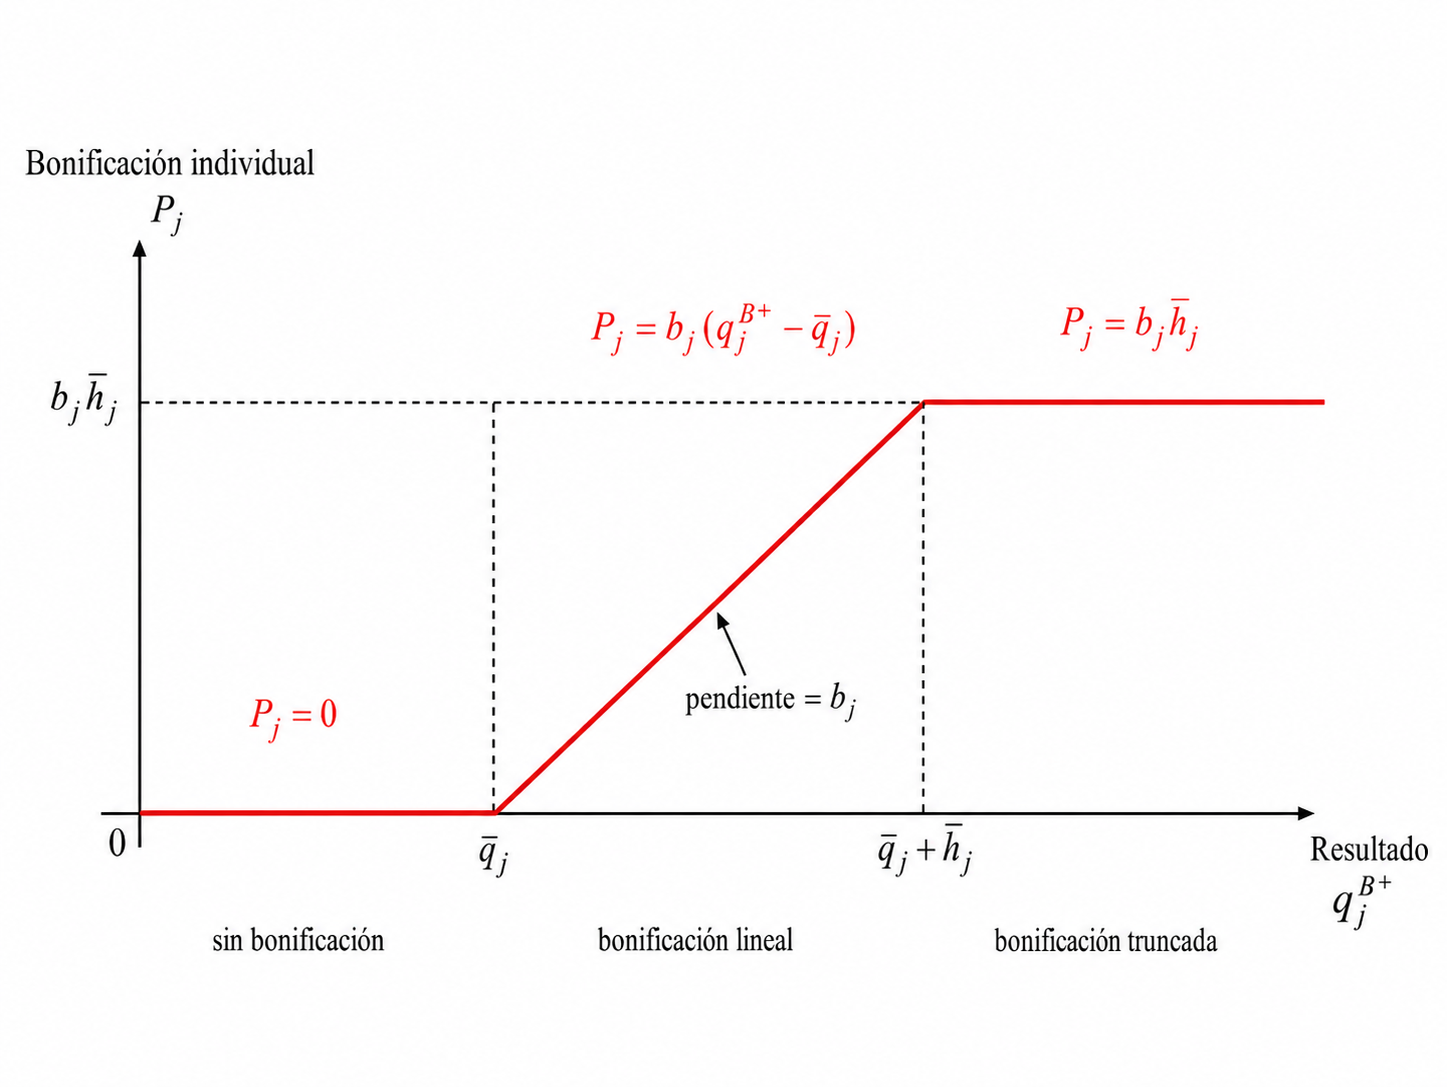
\includegraphics[width=\columnwidth]{figuras/bonif_sobrecumpl.png}

    \vspace{1mm}

    \begin{minipage}{\columnwidth}
        \raggedright
        {\footnotesize
        \textit{Nota:} Para un resultado elegible, la bonificación es nula hasta alcanzar la meta \(\bar q_j\), aumenta dentro del rango reconocido a una tasa \(\kappa_jb_j\) por unidad adicional y queda acotada en \(\kappa_jb_j\bar h_j\). Los parámetros \(b_j\), \(\kappa_j\) y \(\bar h_j\) se determinan ex ante en el estudio tarifario, sujeto a \(\bar q_j+\bar h_j\leq q_j^{\max}\).
        \textit{Fuente:} Elaboración propia.\par}
    \end{minipage}
\end{figure}

El monto reconocido mediante \(T\) se incorpora tarifariamente y permanece afectado al financiamiento de inversiones. Para evitar una doble contabilización, \(S^{B^{+}}\) recoge los recursos que permanecen efectivamente sin utilizar después de ejecutar el alcance que genera el resultado observado, mientras que \(T\) representa el reconocimiento regulatorio asociado con el sobrecumplimiento. Los recursos utilizados para producir el resultado adicional no se contabilizan simultáneamente como ahorro. En el canal reputacional, ambas formas de valor reconocido se consideran conjuntamente mediante \(R_E(S^{B^{+}}+T)\).

\subsubsection{Reputación e incentivo de ejecución bajo \(B^{+}\)}

El esquema \(B^{+}\) conserva las reglas de fiscalización y sanción de \(B\). Las metas de \(J^{G}\) y los indicadores específicos asociados con \(R^{F}\) permanecen fuera del ICG y mantienen sus mecanismos propios de verificación. La modificación se limita al reconocimiento acotado de resultados superiores a las metas.

Se supone que \(T\) no es apropiable por el gerente y no entra como compensación monetaria directa en \(U_G^{B^{+}}\). Su efecto opera únicamente a través de la valoración reputacional de los recursos reconocidos. Como \(B\) concentra la señal publicada en los resultados del servicio, el desempeño percibido bajo la extensión se define como

\begin{equation}
\label{eq:desempeno_percibido_bplus}
P^{B^{+}}
\equiv
C_S
+
\frac{1}{n_S}
\sum_{j\in J^{S}}
\frac{h_j}{\bar q_j}.
\end{equation}

Así, \(P^{B^{+}}=P^B=C_S\) cuando no existe sobrecumplimiento elegible. La reputación se extiende como

\begin{equation}
\label{eq:reputacion_bplus}
\begin{aligned}
\mathrm{Rep}^{B^{+}}
={}&
d_I\ell_I^{B^{+}}
R_I\left(P^{B^{+}}\right)
\\
&+
d_E\ell_E
R_E\left(S^{B^{+}}+T\right)
\\
&-
p\,d_M\ell_M
R_M\left(M^{B^{+}}\right).
\end{aligned}
\end{equation}

Si el regulador publica separadamente el cumplimiento base y el sobrecumplimiento reconocido, se supone \(\ell_I^{B^{+}}=\ell_I^{B}\). Los retornos marginales relevantes para los nuevos canales son

\begin{subequations}
\label{eq:retornos_marginales_bplus}
\begin{align}
\lambda^{B^{+}}
&\equiv
V'\!\left(\mathrm{Rep}^{B^{+}}\right)
d_I\ell_I^{B^{+}}
\notag\\
&\quad\times
R_I'\!\left(P^{B^{+}}\right),
\\
\varpi^{B^{+}}
&\equiv
V'\!\left(\mathrm{Rep}^{B^{+}}\right)
d_E\ell_E
\notag\\
&\quad\times
R_E'\!\left(S^{B^{+}}+T\right).
\label{eq:varpi_bplus}
\end{align}
\end{subequations}

Para aislar el efecto propio del sobrecumplimiento se mantienen localmente constantes los canales sancionadores comunes a ambos esquemas, de modo que \(\gamma^{B^{+}}=\gamma^{B}\). Las comparaciones se realizan dentro de una región en la que \(\zeta_j\) y los demás indicadores discretos permanecen fijos.

Considérese una intervención \(r\in R_j^{S}\). Mientras \(q_j\leq\bar q_j\), \(B^{+}\) coincide con \(B\) respecto del resultado \(j\). La diferencia aparece cuando \(\zeta_j=1\) y \(\bar q_j<q_j<\bar q_j+\bar h_j\). En ese intervalo,

\begin{subequations}
\label{eq:derivadas_sobrecumplimiento_bplus}
\begin{align}
\frac{\partial P^{B^{+}}}{\partial e_r}
&=
\frac{1}{n_S}
\frac{\beta_{rj}}{\bar q_j}
\notag\\
&\quad\times
\frac{\partial F_r}{\partial e_r}
>0,
\label{eq:derivada_p_bplus}
\\
\frac{\partial T}{\partial e_r}
&=
\kappa_j b_j
\beta_{rj}
\notag\\
&\quad\times
\frac{\partial F_r}{\partial e_r}
>0.
\label{eq:derivada_premio_bplus}
\end{align}
\end{subequations}

Para una intervención aún no culminada, \(\partial S_r/\partial e_r=0\). Como la regla sancionadora es común a \(B\) y \(B^{+}\), la diferencia entre los componentes continuos del beneficio marginal de ejecución es

\begin{equation}
\label{eq:incentivo_marginal_bplus}
\begin{aligned}
\mathrm{BM}_{r,e}^{B^{+}}
-
\mathrm{BM}_{r,e}^{B}
&=
\Biggl[
\lambda^{B^{+}}
\frac{1}{n_S\bar q_j}
\\
&\qquad
+
\varpi^{B^{+}}
\kappa_j b_j
\Biggr]
\beta_{rj}
\frac{\partial F_r}{\partial e_r}
\\
&\geq
0.
\end{aligned}
\end{equation}

El primer término recoge el retorno reputacional de reconocer el sobrecumplimiento dentro de \(P^{B^{+}}\) y el segundo la valoración reputacional de la bonificación destinada al financiamiento de inversiones. Ninguno requiere aumentar \(\mu_r^m\). La desigualdad es estricta cuando al menos uno de los nuevos canales tiene valoración positiva y la magnitud física continúa respondiendo al esfuerzo. Una vez alcanzado \(q_j\geq\bar q_j+\bar h_j\), \(h_j\) y \(T_j\) permanecen constantes y estos retornos marginales desaparecen.

La saturación del avance físico sí limita este mecanismo. Mientras \(e_r<e_r^{\mathrm{sat}}\), una mayor ejecución puede elevar \(F_r\), \(q_j\) y el sobrecumplimiento reconocido. Una vez alcanzada la región \(e_r\geq e_r^{\mathrm{sat}}\), \(\partial F_r/\partial e_r=0\) y los retornos marginales de \eqref{eq:derivadas_sobrecumplimiento_bplus} desaparecen por este canal.

\begin{resultadobox}
{Incentivo de ejecución bajo \(B^{+}\)}
\label{res:incentivo_ejecucion_bplus}

Para una intervención \(r\in R_j^{S}\), \(B^{+}\) no reduce el beneficio marginal de ejecución respecto de \(B\). Antes de alcanzar la meta ambos esquemas coinciden; dentro del rango de sobrecumplimiento elegible, \(B^{+}\) añade los retornos reputacional y económico asociados con el resultado adicional. Bajo la comparativa estática de la Subsección~4.1,

\begin{equation}
e_r^{B^{+},*}
\geq
e_r^{B,*}.
\end{equation}

La desigualdad es estricta cuando el reconocimiento modifica efectivamente el margen relevante de decisión, al menos uno de los canales adicionales tiene valoración positiva y la magnitud física continúa respondiendo al esfuerzo. El resultado no requiere una mayor exposición sancionadora que en \(B\).
\end{resultadobox}

\subsubsection{Eficiencia y uso de los recursos}

El esfuerzo de eficiencia \(g_r\) reduce los recursos necesarios para ejecutar una magnitud física dada, pero no eleva directamente \(F_r\), \(q_j\) ni el sobrecumplimiento reconocido cuando \(e_r\) permanece constante. Por tanto, el nuevo canal introducido por \(B^{+}\) no altera directamente el retorno tecnológico de \(g_r\).

Para una intervención completada, y manteniendo localmente constantes el resultado observado y \(T\),

\begin{equation}
\label{eq:incentivo_eficiencia_bplus}
\begin{aligned}
\frac{\partial (S^{B^{+}}+T)}{\partial g_r}
&=
-
\frac{\partial I_r}{\partial g_r}
>0,
\\
\mathrm{BM}_{r,g}^{B^{+}}
&=
\varpi^{B^{+}}
\left(
-
\frac{\partial I_r}{\partial g_r}
\right).
\end{aligned}
\end{equation}

El posible efecto intertemporal de los recursos liberados se rige por el canal descrito en la Subsección~4.3 y no constituye un efecto tecnológico directo de \(g_r\) sobre \(q_j\). Asimismo, como la bonificación se determina mediante parámetros fijados ex ante y a partir del resultado verificable, un mayor gasto no constituye por sí mismo una fuente de mayor reconocimiento.

\subsubsection{Desempeño bajo \(B^{+}\)}

El esquema \(B^{+}\) utiliza la misma función de producción de resultados que \(B\). Cualquier diferencia de desempeño proviene, por tanto, de los incentivos adicionales introducidos por el reconocimiento acotado del sobrecumplimiento y no de una modificación tecnológica ni de una mayor exposición sancionadora.

Bajo las condiciones locales del Resultado~\ref{res:incentivo_ejecucion_bplus}, si la respuesta inducida satisface \(F_r^{B^{+}}\geq F_r^{B}\) para las intervenciones relevantes de \(R^{S}\), la monotonicidad de la función de producción implica el siguiente resultado.

\begin{resultadobox}
{Desempeño bajo \(B^{+}\)}
\label{res:desempeno_bplus}

Bajo las condiciones locales anteriores,

\begin{equation}
\widetilde q_S^{B^{+}}
\geq
\widetilde q_S^{B}.
\end{equation}

La desigualdad es estricta cuando el reconocimiento del sobrecumplimiento induce una mayor ejecución física en al menos una intervención de \(R^{S}\) que contribuye positivamente al resultado correspondiente, sin una reducción compensatoria del desempeño generado por las demás intervenciones. Como \(B^{+}\) no modifica directamente los incentivos sobre \(R^{G}\) y la capacidad gerencial no es una restricción vinculante, se mantiene localmente \(C_G^{B^{+}}=C_G^{B}\). Por tanto,

\begin{equation}
\begin{aligned}
Q^{B^{+}}
&=
Q\!\left(
\widetilde q_S^{B^{+}},
C_G^{B}
\right)
\\
&\geq
Q\!\left(
\widetilde q_S^{B},
C_G^{B}
\right)
=
Q^{B}.
\end{aligned}
\end{equation}
\end{resultadobox}

\subsubsection{Bienestar regulatorio y calibración de la bonificación}

El mayor desempeño potencial de \(B^{+}\) no implica por sí solo una mejora de bienestar. A los componentes definidos en la Subsección~4.3 para una transición \(m\to m'\) se añade ahora el costo regulatorio neto de financiar la bonificación. Sea \(C_T(T)\) dicho costo, con

\begin{equation}
\label{eq:costo_bonificacion_bplus}
C_T(0)=0,
\qquad
C_T'(T)>0.
\end{equation}

La función \(C_T(T)\) recoge únicamente el costo fiscal, financiero o administrativo adicional de otorgar la bonificación, neto de su componente de transferencia, y excluye el gasto de inversión ya incorporado en \(C_I^{B^{+}}\). El caso \(C_T(T)=T\) solo corresponde cuando cada unidad reconocida constituye un costo adicional íntegro y distinto de los recursos contabilizados en \(C_I^{B^{+}}\).

El criterio regulatorio bajo \(B^{+}\) es

\begin{equation}
\label{eq:bienestar_regulador_bplus}
W_R^{B^{+}}
=
\Phi\!\left(
Q^{B^{+}}
\right)
-
C_I^{B^{+}}
-
C_{OM}^{B^{+}}
-
\Omega\!\left(M^{B^{+}}\right)
-
C_T(T),
\end{equation}

donde

\begin{equation}
Q^{B^{+}}
=
Q\!\left(
\widetilde q_S^{B^{+}},
C_G^{B^{+}}
\right).
\end{equation}

Utilizando las definiciones generales de \(\Delta_\Phi^{m,m'}\), \(\Delta_\Omega^{m,m'}\), \(\Delta_I^{m,m'}\) y \(\Delta_{OM}^{m,m'}\) de la Subsección~4.3, se añade

\begin{equation}
\label{eq:delta_p_bplus}
\Delta C_T^{B,B^{+}}
\equiv
C_T(T).
\end{equation}

La diferencia de bienestar se reduce entonces a

\begin{equation}
\label{eq:diferencia_bienestar_bplus_b}
\begin{aligned}
W_R^{B^{+}}
-
W_R^{B}
&=
\Delta_{\Phi}^{B,B^{+}}
+
\Delta_{\Omega}^{B,B^{+}}
\\
&\quad
-
\Delta_{I}^{B,B^{+}}
-
\Delta_{OM}^{B,B^{+}}
-
\Delta C_T^{B,B^{+}}.
\end{aligned}
\end{equation}

La igualdad \(M^{B^{+}}=M^B\) de \eqref{eq:multa_bplus} se refiere a un mismo nivel de cumplimiento. En equilibrio, el mayor esfuerzo inducido por \(B^{+}\) puede reducir las bases sancionadoras y, con ello, generar \(\Delta_\Omega^{B,B^{+}}\geq0\). Este canal puede reforzar la ganancia de bienestar, pero no es necesario para que la extensión resulte preferible.

De \eqref{eq:diferencia_bienestar_bplus_b}, la condición para una mejora regulatoria es

\begin{equation}
\label{eq:condicion_bienestar_bplus}
\Delta_{\Phi}^{B,B^{+}}
+
\Delta_{\Omega}^{B,B^{+}}
>
\Delta_{I}^{B,B^{+}}
+
\Delta_{OM}^{B,B^{+}}
+
\Delta C_T^{B,B^{+}}.
\end{equation}

\begin{resultadobox}
{Bienestar regulatorio bajo \(B^{+}\)}
\label{res:bienestar_bplus}

El hecho de que \(Q^{B^{+}}\geq Q^{B}\) no implica, por sí solo, que \(B^{+}\) domine a \(B\). Si se cumple \eqref{eq:condicion_bienestar_bplus}, entonces

\begin{equation}
W_R^{B^{+}}
>
W_R^{B}.
\end{equation}

Por tanto, \(B^{+}\) constituye una mejora regulatoria únicamente cuando el valor del sobrecumplimiento inducido y de cualquier reducción de la carga efectiva de la multa supera el costo neto de la bonificación y cualquier incremento del gasto de inversión o de los costos de operación y mantenimiento.
\end{resultadobox}

La condición de bienestar proporciona una interpretación económica para la calibración de \(\kappa_j\) y \(\bar h_j\). Un reconocimiento demasiado bajo puede no modificar suficientemente el esfuerzo, mientras que uno excesivamente alto puede elevar \(\Delta C_T^{B,B^{+}}\) por encima del valor regulatorio del desempeño adicional. El límite \(\bar h_j\) evita además que el mecanismo continúe reconociendo resultados una vez agotado el rango que el regulador considera valioso.

La incorporación de \(B^{+}\) al ordenamiento condicionado completo de bienestar se presenta en la Subsección~4.5.


\subsection{Síntesis de resultados}

Las Subsecciones~4.3 y~4.4 muestran que las modificaciones regulatorias afectan de manera distinta la ejecución, los resultados del servicio, el cumplimiento de otras metas, la eficiencia y el bienestar. La secuencia principal \(A\to A'\to A''\to B\) separa progresivamente cambios específicos del diseño; \(A_0\to A\) se mantiene como \textit{benchmark} institucional y \(B\to B^{+}\) incorpora el reconocimiento acotado del sobrecumplimiento. Todos los ordenamientos están sujetos a las condiciones metodológicas y locales establecidas previamente.

La Tabla~\ref{tab:sintesis_resultados_esquemas} resume los resultados sin reproducir sus derivaciones.

\begin{table*}[t]
\centering
\caption{Síntesis de los principales resultados por transición}
\label{tab:sintesis_resultados_esquemas}
\scriptsize
\renewcommand{\arraystretch}{1.35}
\setlength{\tabcolsep}{2.3pt}

\begin{tabularx}{\textwidth}{
@{}
>{\centering\arraybackslash}p{0.075\textwidth}
>{\raggedright\arraybackslash}p{0.205\textwidth}
>{\raggedright\arraybackslash}p{0.17\textwidth}
>{\raggedright\arraybackslash}p{0.19\textwidth}
>{\raggedright\arraybackslash}X
@{}
}
\hline

\textbf{Transición}
&
\textbf{Ejecución y resultados del servicio}
&
\textbf{Cumplimiento de gestión (\(C_G\))}
&
\textbf{Eficiencia}
&
\textbf{Criterio regulatorio}
\\

\hline

\(A_0\to A\)
&
Orden abierto; bajo saturación y \eqref{eq:condicion_focalizacion_a_a0}, \(\widetilde q_S^{A}\geq\widetilde q_S^{A_0}\) (Resultado~\ref{res:desempeno_agregado}).
&
Orden abierto.
&
Mejora débil para \(R^{S}\cup R^{G}\); orden abierto para \(R^{F}\) (Resultado~\ref{res:eficiencia_benchmark_a0_a}).
&
Comparación abierta; evaluar con la descomposición \eqref{eq:cambio_bienestar_transicion}.
\\[5pt]

\(A\to A'\)
&
\(\widetilde q_S^{A'}\geq\widetilde q_S^{A}\) (Resultados~\ref{res:incentivo_ejecucion_rs} y~\ref{res:desempeno_agregado}).
&
\(C_G^{A'}\geq C_G^{A}\) (Resultado~\ref{res:cumplimiento_agregado_g}).
&
Sin cambio para \(R^{S}\cup R^{G}\); \(g_r^{A,*}\geq g_r^{A',*}\) para \(R^{F}\) (Resultado~\ref{res:eficiencia_secuencia_principal}).
&
Evaluar con \eqref{eq:cambio_bienestar_transicion}; no hay orden automático.
\\[5pt]

\(A'\to A''\)
&
\(\widetilde q_S^{A''}\geq\widetilde q_S^{A'}\); ejecución de \(R^{F}\) con orden abierto (Resultado~\ref{res:desempeno_agregado}).
&
\(C_G^{A''}\geq C_G^{A'}\) (Resultado~\ref{res:cumplimiento_agregado_g}).
&
\(g_r^{A'',*}\geq g_r^{A',*}\) para \(R^{F}\) (Resultado~\ref{res:eficiencia_secuencia_principal}).
&
Evaluar con \eqref{eq:cambio_bienestar_transicion}; no hay orden automático.
\\[5pt]

\(A''\to B\)
&
Bajo \eqref{eq:condicion_lambda_b}, \(\widetilde q_S^{B}\geq\widetilde q_S^{A''}\) (Resultado~\ref{res:desempeno_agregado}).
&
\(C_G^{A''}\geq C_G^{B}\) (Resultado~\ref{res:cumplimiento_agregado_g}).
&
Sin cambio bajo las normalizaciones locales.
&
Comparación abierta; debe incluir la oposición entre \(\widetilde q_S\) y \(C_G\).
\\[5pt]

\(B\to B^{+}\)
&
\(\widetilde q_S^{B^{+}}\geq\widetilde q_S^{B}\) y \(Q^{B^{+}}\geq Q^{B}\) (Resultado~\ref{res:desempeno_bplus}).
&
Sin canal directo adicional.
&
Sin efecto tecnológico directo de \(g_r\) sobre el sobrecumplimiento o la bonificación.
&
Evaluar con \eqref{eq:condicion_bienestar_bplus}, incluido el costo neto de la bonificación.
\\

\hline
\end{tabularx}

\vspace{1mm}

\begin{minipage}{0.98\textwidth}
\raggedright
\footnotesize
\textit{Nota:} Los ordenamientos se interpretan bajo las condiciones locales de las Subsecciones~4.1--4.4. Las comparaciones de bienestar del modelo base remiten a \eqref{eq:condicion_general_mejora_bienestar}; la extensión \(B^{+}\) incorpora además el costo neto de la bonificación.
\end{minipage}

\end{table*}

La tabla no implica la cadena \(W_R^{B^{+}}>W_R^{B}>W_R^{A''}>W_R^{A'}>W_R^{A}>W_R^{A_0}\). Esa cadena solo podría sostenerse después de verificar empíricamente o mediante supuestos adicionales que cada transición genera una ganancia neta positiva. El modelo identifica los canales y sus signos locales, pero deja abierto el orden global del criterio regulatorio.

En conjunto, el modelo separa progresivamente tres funciones que en los diseños iniciales aparecen parcialmente superpuestas: la evaluación regulatoria mediante el \(ICG^m\), la señal reputacional resumida por \(P^m\) y la estructura de consecuencias. La salida de componentes del ICG reasigna mecánicamente sus ponderaciones regulatorias, mientras que la composición de \(P^m\) determina, a partir de las saliencias \(s_H\), el peso reputacional de los bloques que permanecen. Esta separación puede corregir distorsiones, pero no implica que todas las transiciones mejoren simultáneamente todos los márgenes. Un diseño puede fortalecer los incentivos de una tarea específica o elevar los resultados directos del servicio y, aun así, no mejorar el bienestar regulatorio. Esta última conclusión exige que el efecto conjunto sobre \(Q(\widetilde q_S,C_G)\), el gasto efectivo de inversión, los costos de operación y mantenimiento y la carga sectorial de las multas sea favorable. En consecuencia, incluso cuando \(B^{+}\) eleva el desempeño potencial, su posición en el criterio regulatorio depende del costo de la bonificación, de los recursos adicionales y de la carga sancionadora. La comparación debe realizarse transición por transición.

\section{Discusión de resultados e implicancias para el diseño regulatorio}
\label{sec:implicancias_regulatorias}

Esta sección interpreta conjuntamente los resultados del análisis y examina sus implicancias para el diseño regulatorio de las metas de gestión. El objetivo no es derivar una arquitectura óptima ni formular una propuesta de implementación inmediata, sino identificar qué aspectos del diseño vigente resultan afectados por los mecanismos examinados, qué modificaciones encuentran mayor respaldo en el modelo y bajo qué condiciones podrían ser consideradas.

Los resultados no atribuyen una misma conclusión a todas las transiciones. La focalización de la medición financiera mejora la separación entre instrumentos, aunque su efecto sobre la ejecución contemporánea permanece condicionado; la eliminación del umbral agregado impide que el cumplimiento en otras dimensiones desactive consecuencias asociadas con incumplimientos ya configurados; la sustitución de la verificación financiera por indicadores físicos o funcionales evita que una reducción eficiente del gasto sea tratada, por sí sola, como menor cumplimiento de las intervenciones de \(R^{F}\); y la delimitación del ICG concentra su contenido informativo en los resultados que se pretende hacer visibles. Estas diferencias aconsejan discutir las implicancias de cada modificación por separado, antes que tratarlas como un paquete regulatorio indivisible.

La secuencia \(A_{0}\rightarrow A\rightarrow A'\rightarrow A''\rightarrow B\) cumple, por tanto, una función analítica. Permite identificar el mecanismo asociado con cada cambio y distinguir entre efectos sobre la ejecución, la eficiencia y la señal reputacional. La extensión \(B^{+}\) tiene un estatuto distinto: no corrige una superposición entre instrumentos, sino que incorpora un reconocimiento acotado del sobrecumplimiento y, por ello, requiere condiciones de elegibilidad y salvaguardas propias.


\subsection{Interpretación conjunta de los resultados}
\label{subsec:discusion_resultados}

La transición \(A_{0}\rightarrow A\) focaliza el avance financiero en las intervenciones de \(R^{F}\) y retira la relación de trabajo del ICG y de las consecuencias pecuniarias. Para las inversiones de \(R^{S}\) y \(R^{G}\), la focalización elimina su participación en el avance financiero general y, con ello, la posibilidad de que una reducción eficiente del costo deteriore la señal financiera o aumente la consecuencia asociada con dicho avance. Al mismo tiempo, la salida de la relación de trabajo elimina otra vía mediante la cual una misma inversión podía incidir en el índice y en la base de las consecuencias. Esta mayor separación no implica, sin embargo, un aumento incondicional del esfuerzo contemporáneo de ejecución: la transición modifica simultáneamente varios canales, por lo que el modelo no establece un orden general entre \(e_r^{A_0,*}\) y \(e_r^{A,*}\). Para las intervenciones de \(R^{S}\) y \(R^{G}\), en cambio, la focalización sí elimina los canales financieros que podían penalizar una reducción eficiente del costo, de modo que el incentivo de eficiencia no se debilita y puede aumentar cuando alguno de esos canales se encontraba activo.

La transición \(A\rightarrow A'\) modifica la regla de activación de las consecuencias pecuniarias. El ICG conserva la misma composición y las intervenciones de \(R^{F}\) continúan verificándose mediante el avance financiero focalizado, pero el umbral agregado deja de determinar si los incumplimientos ya configurados generan una consecuencia. Bajo \(A\), un valor \(ICG^{A}\geq\tau\) puede desactivar conjuntamente las consecuencias pese a que subsistan obligaciones incumplidas; desde \(A'\), cada componente conserva su consecuencia mientras permanezca configurado el incumplimiento correspondiente. Esta modificación puede fortalecer el incentivo de ejecución cuando el umbral habría mantenido inactivo el canal sancionador. Para \(R^{F}\), sin embargo, también puede reducir el incentivo de eficiencia al hacer efectiva una consecuencia financiera que bajo \(A\) podía encontrarse desactivada. La eliminación del umbral no sustituye el análisis de imputabilidad ni la necesidad de que la obligación y la conducta sancionable se encuentren previamente identificadas.

La transición \(A'\rightarrow A''\) sustituye la verificación financiera de \(R^{F}\) por indicadores específicos de cumplimiento físico o funcional de \(J^{F}\). El avance financiero focalizado deja de formar parte del ICG y de la base utilizada para determinar las consecuencias de estas intervenciones. En su lugar, el incumplimiento se verifica directamente mediante el indicador aplicable y la cuantificación se vincula con el alcance físico pendiente. Para las intervenciones de \(R^{S}\), la salida de \(f_F\) aumenta el peso de \(C_S\) dentro del ICG y fortalece su incentivo de ejecución. Para \(R^{F}\), el efecto sobre la ejecución es, en general, ambiguo, porque desaparecen tanto el retorno reputacional asociado con elevar el gasto como la reducción de la base financiera, mientras aparece el canal asociado con la base física. El efecto sobre la eficiencia es más definido: al retirarse los canales que penalizaban una reducción del gasto, \(A''\) no debilita y puede fortalecer el incentivo de eficiencia respecto de \(A'\).

La transición \(A''\rightarrow B\) completa la delimitación de la señal agregada. Al retirar \(C_G\) del ICG, el índice queda definido exclusivamente por \(C_S\), esto es, por el cumplimiento de los resultados comprendidos en \(J^{S}\). Para las inversiones de \(R^{S}\), esta modificación puede fortalecer el retorno reputacional del esfuerzo cuando la mayor concentración del índice en resultados incrementa suficientemente su legibilidad y valoración. Para las intervenciones de \(R^{G}\), en cambio, desaparece el retorno reputacional asociado con \(C_G\), aunque sus consecuencias específicas permanecen vigentes. Las intervenciones de \(R^{F}\) no modifican su tratamiento en esta transición, pues desde \(A''\) se encuentran fuera del ICG y sujetas a sus indicadores específicos de cumplimiento físico o funcional.

En conjunto, los resultados no establecen un ordenamiento global \(B\succ A_{0}\) para todos los márgenes de decisión. El aporte del modelo consiste, más bien, en identificar qué problema corrige cada transición y qué efectos puede producir sobre distintos incentivos. Esta lectura es especialmente importante para la discusión regulatoria: una modificación puede mejorar la congruencia entre objeto e instrumento sin aumentar necesariamente todos los esfuerzos observados, y un incentivo más intenso no es por sí mismo evidencia de una mejor arquitectura si proviene de una métrica que premia gasto redundante o penaliza eficiencia.


\subsection{Implicancias para la composición y función del ICG}
\label{subsec:implicancias_icg}

Si el ICG debe cumplir principalmente una función informativa y reputacional después de la desvinculación de los incrementos tarifarios base, los resultados sugieren que su composición debería partir del concepto que se pretende representar. Bajo la alternativa analizada, \(J^{S}\) comprende indicadores que miden directamente condiciones observables de cobertura y calidad del servicio, mientras que las inversiones, actividades, capacidades de gestión y demás medios utilizados para producirlas permanecen sujetos a instrumentos específicos.

Esta delimitación debe realizarse a partir del objeto directamente medido por cada indicador y no únicamente de su ubicación normativa dentro del SIIGEPSS. Los aspectos de cobertura y calidad pueden contener, junto con resultados propiamente dichos, variables que verifican ejecución física o funcional. Del mismo modo, indicadores de eficiencia empresarial como la relación de trabajo o el agua no facturada pueden ser relevantes para la supervisión y para la sostenibilidad de la prestación sin constituir, por ese solo hecho, resultados de \(J^{S}\). Su eventual exclusión del ICG no implicaría dejar de medirlos, sino separar su función de seguimiento de la señal agregada de desempeño.

La micromedición requiere una clasificación particularmente cuidadosa. Cuando el indicador verifica principalmente la instalación efectiva de medidores o el cumplimiento de un alcance físico identificable, su naturaleza se aproxima a una obligación de implementación y no a un resultado final de \(J^{S}\). Cuando, en cambio, se utilice un indicador que represente una condición operativa más amplia, su tratamiento deberá depender del objeto efectivamente medido. La pertenencia formal a una categoría normativa no debería sustituir esta evaluación funcional.

Las demás metas de gestión y dimensiones regulatorias pueden conservar reportes, metas, mecanismos de supervisión y, cuando corresponda, consecuencias autónomas. \(C_G\) resume en el modelo las metas de gestión distintas de los resultados del servicio, mientras que otros indicadores, como la relación de trabajo, el agua no facturada, los indicadores de sostenibilidad, solvencia, gobernanza, cumplimiento normativo o focalización del subsidio, pueden proporcionar información valiosa para fines específicos aun cuando no formen parte de \(C_S\). El cambio examinado consiste en evitar que todos ellos modifiquen automáticamente una medida destinada a resumir resultados de cobertura y calidad.

La utilidad de un ICG concentrado en resultados depende, además, de la difusión y legibilidad de la señal. Si el canal reputacional representado por \(d_I\) y \(\ell_I^{m}\) es débil, retirar componentes del índice no garantiza por sí mismo una respuesta gerencial relevante. Una eventual reforma tendría que acompañarse, por tanto, de una política de publicación que permita comparar resultados entre empresas y a lo largo del tiempo, mostrar los componentes del índice y distinguir con claridad el desempeño agregado de los demás indicadores regulatorios.

La evaluación individual y territorial debería mantenerse como complemento de la señal agregada. El ICG no sustituye la identificación del indicador específico incumplido ni la información necesaria para interpretar brechas entre localidades. La separación propuesta afecta la función del agregado, no la disponibilidad de información desagregada para fines de supervisión, transparencia o adopción de medidas correctivas.

La ponderación de los componentes también requiere una decisión explícita. Cuando el ICG se construye como un promedio simple, el número de metas asignadas a una dimensión determina implícitamente su incidencia agregada. Si se adopta una medida destinada a representar resultados de desempeño, la selección de ponderadores debería responder a un marco conceptual explícito y no únicamente a la cantidad de indicadores incluidos en cada estudio tarifario. Esta decisión es distinta de la valoración económica utilizada para determinar sanciones o reconocimientos y no tiene por qué reproducirla.


\subsection{Implicancias para la fiscalización y el régimen sancionador}
\label{subsec:implicancias_fiscalizacion_sanciones}

La exclusión de una inversión o de otra obligación de implementación del ICG no reduce su exigibilidad. Las intervenciones de \(R^{S}\), \(R^{G}\) y \(R^{F}\) continuarían sujetas a programación, seguimiento, fiscalización y, cuando exista una obligación autónoma, atribuible y expresamente tipificada, a medidas correctivas o consecuencias sancionadoras. La diferencia es que su tratamiento debe guardar correspondencia con el objeto de la obligación y no depender necesariamente de su incidencia dentro de una medida agregada de desempeño.

El Programa de Ejecución de Metas Físico-Financieras ofrece una base institucional para esta separación. Como instrumento de trazabilidad, puede vincular cada inversión o medida de mejora con su alcance, presupuesto, fuente de financiamiento, fases de ejecución, hitos, fecha prevista de entrada en operación, riesgos y medidas de contingencia. Esta información permitiría distinguir entre retrasos atribuibles, cambios de programación compatibles con el marco regulatorio y circunstancias externas que requieran un tratamiento específico.

Los resultados del modelo respaldan una distinción entre tres dimensiones que no deberían confundirse: alcance físico o funcional, costo y entrada efectiva en operación. El gasto realizado no acredita por sí mismo que el alcance haya sido completado; una inversión puede culminarse a un costo inferior al presupuesto; y una obra formalmente terminada puede no encontrarse todavía operativa. La fiscalización puede utilizar conjuntamente información financiera, física y funcional, pero la variable empleada para determinar el cumplimiento debería guardar correspondencia con la obligación efectivamente exigida.

El caso de EPS SEDA HUÁNUCO S.A., desarrollado en la discusión de los problemas de activación sancionadora de la Sección~3, ilustra la relevancia de esta distinción. La intervención examinada completó su alcance por debajo del presupuesto y el ahorro fue excluido de la base utilizada para determinar la multa, aunque el menor gasto continuó reduciendo el indicador financiero. En la representación del modelo, este problema corresponde al tratamiento de las intervenciones de \(R^{F}\): \(A\) y \(A'\) mantienen la verificación financiera focalizada, mientras que \(A''\) y \(B\) la sustituyen por indicadores específicos de cumplimiento físico o funcional. La implicancia no es que todo menor gasto constituya eficiencia, sino que un costo inferior no debería interpretarse por sí mismo como menor cumplimiento cuando se hayan preservado el alcance, la calidad, la capacidad, la vida útil y las demás condiciones exigibles.

La separación de instrumentos también obliga a revisar la relación entre el umbral agregado y las obligaciones específicas. Si una obligación permanece incumplida, el modelo muestra que condicionar su consecuencia al valor de un índice que agrega otras metas puede generar una zona en la que el mayor cumplimiento de unas dimensiones neutralice el incumplimiento de otras. La transición \(A\rightarrow A'\) elimina precisamente esta condición de activación. Esto justifica examinar si el umbral del ICG debe continuar operando como activador de consecuencias asociadas con obligaciones individualizables. La revisión no implica que toda brecha inferior al 100~\% deba sancionarse automáticamente: razones de materialidad, error de medición, costos de fiscalización o causas no atribuibles pueden justificar tolerancias o exclusiones, pero deberían tratarse mediante reglas congruentes con la obligación específica.

La imputabilidad conserva un papel central. Las causales previstas en el numeral 30.2 del Reglamento General de Fiscalización y Sanción permiten valorar circunstancias como caso fortuito, fuerza mayor, hecho determinante de tercero u otras situaciones previstas por la normativa. Bajo una arquitectura de obligaciones específicas, este análisis operaría después de verificar la existencia de la brecha y antes de atribuir responsabilidad. De este modo, separar la consecuencia del ICG no equivale a convertir automáticamente cualquier incumplimiento físico en responsabilidad administrativa.

La base económica de la sanción debería guardar correspondencia con la conducta tipificada y evitar valorizaciones repetidas. Cuando una misma inversión contribuya a varios resultados o se encuentre relacionada con varias metas, su valor no debería contabilizarse íntegramente más de una vez dentro de la consecuencia económica. El Anexo~\ref{app:calculo_sancionador} desarrolla esta correspondencia para las inversiones no ejecutadas. Esta cuestión es distinta del \textit{non bis in idem}: la duplicación de una base económica puede ocurrir incluso dentro de una sola multa, mientras que el principio de \textit{non bis in idem} controla la imposición de más de una sanción por una misma conducta cuando concurren las identidades exigidas por la normativa.

Los incumplimientos de resultados de \(J^{S}\) requieren una lógica propia. Una meta de desempeño puede generar la consecuencia específica prevista para su incumplimiento sin que esta dependa del valor agregado del ICG. Además, una misma dimensión puede encontrarse sujeta a un estándar normativo autónomo de continuidad, presión, calidad, acceso u otra condición de la prestación. En ese caso, la consecuencia debería responder a la afectación producida, al beneficio ilícito o a otra base económica congruente con la obligación incumplida, y no reutilizar automáticamente el costo de una inversión ya considerado dentro del control del programa de inversiones.

La misma lógica se extiende a las demás metas de gestión y a los indicadores operativos que permanecen fuera de \(C_S\). La relación de trabajo, el agua no facturada u otros indicadores pueden conservar exigibilidad cuando exista una obligación autónoma, pero su eventual fiscalización debe corresponder a la conducta que representan. No resulta necesario reproducir para ellos la metodología de alcance físico aplicable a una intervención discreta cuando su producción depende de decisiones continuas de operación, gestión comercial, organización e inversión.

Las dificultades descritas pueden reducirse mediante una tipificación vinculada directamente con el incumplimiento atribuible del programa de inversiones. Bajo este enfoque, la conducta sancionable sería la falta de ejecución oportuna de una inversión previamente identificada, programada y financiada.

La obligación incumplida correspondería a la inversión \(r\); el monto relevante sería \(U_r\), construido conforme al procedimiento de determinación del monto dejado de invertir desarrollado en el Anexo~\ref{app:calculo_sancionador}; y la consecuencia económica se calcularía a partir de su costo postergado \(CP_r\), definido en la ecuación~\eqref{eq:anexo_costo_postergado}. De este modo, cada inversión sería valorada una sola vez, con independencia del número de metas o indicadores a los que contribuya.

Esta formulación establece una correspondencia directa entre la conducta tipificada, la base económica y la sanción. Asimismo, elimina la necesidad de reconstruir índices individuales hipotéticos para distribuir la brecha de un ICG agregado cuando la obligación incumplida puede identificarse directamente en el programa de inversiones.

La tipificación basada en inversiones no impide mantener estándares ni consecuencias específicas frente a incumplimientos autónomos de los resultados del servicio. Si una reducción de la continuidad, la presión, la calidad del agua u otro indicador genera una afectación independiente a los usuarios, dicha conducta puede evaluarse mediante medidas correctivas o tipificaciones específicas de calidad. En ese supuesto, la consecuencia regulatoria debe guardar relación con la afectación producida y no reutilizar como base económica la inversión ya considerada en el incumplimiento del programa.

En síntesis, la metodología basada en índices parte del incumplimiento de una meta o de un indicador agregado y posteriormente identifica las inversiones vinculadas con dicho incumplimiento. Este procedimiento resulta relativamente directo cuando existe una relación clara entre una meta y una inversión, pero se vuelve más complejo cuando la infracción se configura mediante el ICG o cuando existen inversiones compartidas. Una tipificación centrada en el programa de inversiones permitiría identificar directamente cada obligación incumplida, valorar una sola vez su postergación y reducir la necesidad de reconstrucciones contrafactuales y asignaciones convencionales.


\subsection{Condiciones para una eventual implementación}
\label{subsec:condiciones_eventual_implementacion}

Las implicancias anteriores no determinan por sí mismas una reforma inmediata. Una eventual implementación requeriría, en primer lugar, revisar el sistema de indicadores para clasificar cada variable según el objeto predominantemente medido: resultado de \(J^{S}\), intervención vinculada con \(R^{S}\), \(R^{G}\) o \(R^{F}\), indicador de eficiencia empresarial u otro propósito regulatorio especializado. Esta revisión permitiría evitar que la ubicación normativa de un indicador determine automáticamente su tratamiento dentro del ICG.

En segundo lugar, las obligaciones de implementación tendrían que encontrarse suficientemente individualizadas. Para fiscalizar separadamente una inversión, actividad o medida de mejora es necesario identificar su alcance exigible, plazo, hitos, medios de verificación, condiciones de entrada en operación, presupuesto o referencia económica y tratamiento de causas no atribuibles. La separación del ICG solo es sostenible si el instrumento alternativo de control conserva trazabilidad suficiente.

En tercer lugar, sería necesario asegurar la consistencia entre los estudios tarifarios vigentes, las reglas de fiscalización y las tipificaciones. La transición plantea una dificultad especial porque pueden coexistir estudios aprobados con metas de avance financiero de alcance amplio y otros sujetos a la focalización introducida posteriormente. Cualquier modificación adicional debería definir expresamente el tratamiento de las obligaciones ya aprobadas y evitar alterar retroactivamente las condiciones bajo las cuales se fijaron tarifas, metas y programas de inversión.

En cuarto lugar, la utilidad de un ICG predominantemente reputacional depende de la calidad de la información y de su difusión. La separación de componentes solo mejora la señal si el regulador publica resultados de manera oportuna, comparable y comprensible, y si los actores relevantes pueden distinguir entre desempeño, ejecución de inversiones y otras dimensiones de gestión. Sin esta condición, la mejora en la composición formal del índice podría no traducirse en un incentivo reputacional material.

En quinto lugar, la reforma del régimen sancionador requeriría información que permita relacionar cada obligación con el alcance pendiente, el presupuesto reconocido, el estado de ejecución, la entrada en operación y las causas del retraso. Sin esa trazabilidad, sustituir una regla agregada por consecuencias individualizadas podría aumentar la discrecionalidad o los costos de fiscalización. La separación de instrumentos exige, por tanto, capacidad administrativa suficiente para sostener el mayor grado de identificación que propone.

La secuencia \(A_{0}\rightarrow A\rightarrow A'\rightarrow A''\rightarrow B\) no debe interpretarse como un calendario obligatorio de reforma. \(A_{0}\rightarrow A\) reconstruye una modificación normativa que focaliza el avance financiero y, en la representación analítica, retira la relación de trabajo del ICG y de las consecuencias pecuniarias; las transiciones posteriores constituyen comparaciones de diseño. La implementación podría ser gradual y no necesariamente reproducir exactamente el orden del modelo, pero cualquier combinación debería preservar la coherencia entre medición, fiscalización y sanción. En particular, excluir obligaciones del ICG sin asegurar previamente su seguimiento y exigibilidad separada podría debilitar el incentivo de ejecución.


\subsection{Tratamiento del sobrecumplimiento}
\label{subsec:implicancias_bonificacion}

La extensión \(B^{+}\) debe interpretarse separadamente de las modificaciones anteriores. Mientras \(A_{0}\rightarrow B\) analiza la congruencia entre objetos e instrumentos, \(B^{+}\) incorpora un incentivo adicional destinado a reconocer resultados verificables por encima de la meta. Su eventual utilización requiere, por tanto, una evaluación específica y no constituye una consecuencia necesaria de delimitar el ICG.

El cumplimiento ordinario puede continuar truncándose en 100~\%, de modo que el componente base \(C_S\) no permita que el sobrecumplimiento de una meta eleve el cumplimiento ordinario de otra. \(B^{+}\) identifica separadamente el desempeño adicional y lo incorpora de manera acotada al ICG extendido, además de asociarle, cuando corresponda, una bonificación predeterminada. Como las consecuencias específicas dejan de depender del nivel agregado del ICG desde \(A'\), el sobrecumplimiento reconocido no desactiva incumplimientos ni consecuencias correspondientes a otras obligaciones.

La selección de los resultados elegibles tendría que considerar, entre otros elementos, la relevancia para los usuarios, la controlabilidad, la verificabilidad, la sostenibilidad de la mejora y la posibilidad de atribuirla razonablemente a las decisiones de la empresa. También deberían definirse ex ante el rango máximo de sobrecumplimiento reconocido, la valoración aplicable por unidad adicional y las condiciones que excluyen el reconocimiento cuando el resultado responde principalmente a factores externos.

El modelo abstrae de restricciones vinculantes de capacidad gerencial y supone costos separables entre intervenciones para aislar el efecto del reconocimiento del sobrecumplimiento. Bajo esos supuestos, \(B^{+}\) no desplaza mecánicamente esfuerzo desde otras actividades y puede mantener un retorno marginal positivo una vez alcanzada la meta, dentro del rango reconocido. En la práctica, sin embargo, una capacidad gerencial o unos recursos limitados podrían generar reasignaciones desde obligaciones todavía pendientes. Este riesgo queda fuera del alcance formal del modelo y debería considerarse al diseñar las reglas de elegibilidad y los límites del mecanismo.

El reconocimiento puede ser reputacional, regulatorio o económico. Una modalidad reputacional resulta consistente con la función informativa del ICG y puede implementarse mediante publicaciones, comparaciones o reconocimientos diferenciados. Una modalidad económica exigiría una evaluación adicional de financiamiento, incidencia tarifaria, distribución de beneficios entre empresa y usuarios y límites por indicador o periodo. En ningún caso el reconocimiento debería restablecer automáticamente la condicionalidad general de los incrementos tarifarios base ni operar como mecanismo de compensación de incumplimientos en otras dimensiones.

La gradualidad es particularmente relevante para \(B^{+}\). Antes de introducir una bonificación económica generalizada, podría evaluarse un conjunto acotado de indicadores con información suficientemente robusta, reglas de elegibilidad predeterminadas y mecanismos para verificar persistencia y atribución. La continuidad o ampliación del mecanismo debería depender de que la evidencia obtenida permita distinguir mejoras adicionales de variaciones transitorias o de resultados producidos principalmente por factores externos.

En síntesis, las implicancias del análisis apuntan menos a la adopción de un paquete cerrado que a una separación funcional entre objetos regulatorios. El ICG puede concentrarse en los resultados de \(J^{S}\); las intervenciones de \(R^{S}\), \(R^{G}\) y \(R^{F}\) pueden permanecer sujetas a programación, fiscalización y consecuencias específicas conforme a la naturaleza de cada obligación; los demás indicadores regulatorios pueden conservar mecanismos especializados de seguimiento; y el sobrecumplimiento puede tratarse, si se justifica, mediante un componente adicional y acotado. La conveniencia de cada modificación depende de las condiciones de información, controlabilidad, atribución y capacidad institucional desarrolladas en esta sección.


\begin{figure*}[t]
\centering

\begin{tikzpicture}[
font=\small,
cadena/.style={
    draw,
    rounded corners=2pt,
    align=center,
    minimum height=2.25cm,
    text width=0.155\textwidth,
    inner sep=5pt
},
instrumento/.style={
    draw,
    rounded corners=2pt,
    align=center,
    minimum height=1.65cm,
    text width=0.155\textwidth,
    inner sep=5pt
},
flecha/.style={
    -{Latex},
    thick
},
control/.style={
    -{Latex},
    densely dashed,
    thick
},
frontera/.style={
    draw,
    dashed,
    rounded corners=4pt,
    inner sep=5pt
}
]

% Cadena principal
\node[cadena] (recursos) {
\textbf{Recursos}\\[2mm]
Recursos tarifarios y fuentes de financiamiento
};

\node[cadena, right=5mm of recursos] (implementacion) {
\textbf{Obligaciones de implementación}\\[2mm]
Inversiones, actividades y medidas de mejora\\[1mm]
\(\left(R^{S}\mathbin{\dot\cup}R^{G}\mathbin{\dot\cup}R^{F}\right)\)
};

\node[cadena, right=5mm of implementacion] (operacion) {
\textbf{Alcance y operación}\\[2mm]
Alcance físico o funcional completado y entrada efectiva en operación
};

\node[cadena, right=5mm of operacion] (resultados) {
\textbf{Resultados de desempeño}\\[2mm]
Cobertura y calidad del servicio\\[1mm]
\(\left(J^{S}\right)\)
};

\node[cadena, right=5mm of resultados] (sobrecumplimiento) {
\textbf{Desempeño adicional}\\[2mm]
Sobrecumplimiento verificable y acotado
};

% Flechas de la cadena
\draw[flecha]
(recursos.east) -- (implementacion.west);

\draw[flecha]
(implementacion.east) -- (operacion.west);

\draw[flecha]
(operacion.east) --
node[
    above,
    align=center,
    font=\scriptsize
] {contribución productiva,\\no equivalencia automática}
(resultados.west);

\draw[flecha]
(resultados.east) -- (sobrecumplimiento.west);

% Frontera del ICG base
\node[
    frontera,
    fit=(resultados),
    label={
        [font=\scriptsize]
        above:\textbf{ICG base de desempeño}
    }
] (icgbox) {};

% Instrumentos regulatorios
\node[instrumento, below=1.65cm of recursos] (seguimiento) {
\textbf{Programación y seguimiento}\\[2mm]
Programación físico-financiera, cronogramas, hitos y alertas
};

\node[instrumento, below=1.65cm of implementacion] (fiscalizacion) {
\textbf{Fiscalización de obligaciones}\\[2mm]
Verificación del cumplimiento y análisis de atribuibilidad
};

\node[instrumento, below=1.65cm of operacion] (verificacion) {
\textbf{Verificación física y funcional}\\[2mm]
Culminación, calidad técnica y entrada efectiva en operación
};

\node[instrumento, below=1.65cm of resultados] (evaluacion) {
\textbf{Evaluación del desempeño}\\[2mm]
ICG, componentes y publicación de resultados
};

\node[instrumento, below=1.65cm of sobrecumplimiento] (bonificacion) {
\textbf{Reconocimiento adicional}\\[2mm]
Componente acotado y bonificación bajo \(B^{+}\)
};

% Flechas verticales
\draw[control]
(seguimiento.north) -- (recursos.south);

\draw[control]
(fiscalizacion.north) -- (implementacion.south);

\draw[control]
(verificacion.north) -- (operacion.south);

\draw[control]
(evaluacion.north) -- (resultados.south);

\draw[control]
(bonificacion.north) -- (sobrecumplimiento.south);

% Etiquetas laterales
\node[
    rotate=90,
    font=\footnotesize\bfseries,
    left=7mm of recursos
] {Cadena de producción};

\node[
    rotate=90,
    font=\footnotesize\bfseries,
    left=7mm of seguimiento
] {Instrumento regulatorio};

\end{tikzpicture}

\caption{Cadena de resultados y separación funcional de instrumentos regulatorios}
\label{fig:cadena_resultados_instrumentos}

\begin{minipage}{0.97\textwidth}
\footnotesize
\textit{Nota:} Las flechas horizontales representan la cadena mediante la cual los recursos y las obligaciones de implementación contribuyen a producir resultados. Esta relación no implica equivalencia entre la ejecución de los medios y la obtención del desempeño. El ICG base se concentra en los resultados comprendidos en \(J^{S}\), mientras que las intervenciones de \(R^{S}\), \(R^{G}\) y \(R^{F}\) permanecen sujetas a programación, seguimiento, fiscalización y, cuando corresponda, consecuencias específicas. Otras dimensiones regulatorias que no se representan en la cadena principal conservan mecanismos especializados de seguimiento y supervisión. Bajo \(B^{+}\), el sobrecumplimiento se identifica mediante un componente adicional y acotado del ICG extendido y puede recibir una bonificación predeterminada, sin modificar el cumplimiento base ni desactivar consecuencias correspondientes a otras obligaciones. \textit{Fuente:} Elaboración propia sobre la base de \citet{oecd2023glossary}, \citet{behn2003measure} y la experiencia regulatoria revisada en el Anexo~\ref{anexo:experiencia_internacional}.
\end{minipage}

\end{figure*}
\section{Conclusiones}

Este estudio examina el diseño de las metas de gestión en la regulación peruana de los servicios de agua potable y saneamiento. El problema central es que el Índice de Cumplimiento Global (ICG) puede combinar indicadores que miden objetos regulatorios distintos: resultados observables de la prestación, variables de eficiencia o gestión, obligaciones de implementación y ejecución financiera de inversiones o reservas. Esta composición no es neutral, pues condiciona tanto la interpretación del índice como los incentivos que transmite a la empresa prestadora.

La revisión del marco regulatorio y la evidencia de las fiscalizaciones realizadas por la Sunass durante 2024 muestran una marcada heterogeneidad entre las metas evaluadas. El cumplimiento promedio general asciende a 71\%, mientras que los menores niveles se concentran principalmente en metas vinculadas con inversiones, reservas y otras obligaciones de ejecución. Esta evidencia es descriptiva y no identifica causalmente las razones de las diferencias observadas, pero muestra que un mismo porcentaje de incumplimiento puede contener información distinta según la naturaleza del objeto medido, su horizonte temporal y los factores que condicionan su ejecución.

A partir de esta heterogeneidad, el análisis distingue entre los resultados de desempeño comprendidos en \(J^{Q}\), las inversiones vinculadas con su producción, \(R^{Q}\), las demás obligaciones discretas de implementación, \(R^{O}\), y los indicadores de gestión agrupados en \(C^{O}\), cuya tecnología de producción no se representa mediante una inversión específica. Esta clasificación permite separar analíticamente la medición de los resultados, la verificación de las obligaciones de implementación y el seguimiento de otras dimensiones regulatorias sin restar relevancia ni exigibilidad a ninguna de ellas.

La comparación secuencial \(A_{0}\rightarrow A\rightarrow A'\rightarrow A''\rightarrow B\) muestra que los problemas identificados corresponden a mecanismos distintos. La transición \(A_{0}\rightarrow A\) focaliza la medición financiera y elimina, para las inversiones de \(R^{Q}\), la superposición entre su contribución a los resultados y su ejecución financiera dentro del índice, aunque ello no garantiza por sí mismo un mayor esfuerzo contemporáneo de ejecución. La transición \(A\rightarrow A'\) sustituye la ejecución financiera por el alcance físico o funcional como base de verificación de \(R^{O}\) y evita que una inversión completada por debajo del presupuesto continúe siendo tratada como incumplida por el solo hecho de generar un ahorro.

La transición \(A'\rightarrow A''\) corrige un mecanismo diferente. Cuando la consecuencia asociada con las inversiones depende de un umbral agregado del ICG, el cumplimiento de unas dimensiones puede desactivar la sanción aun cuando subsistan obligaciones pendientes. Las sanciones independientes preservan, en cambio, la consecuencia asociada con cada inversión mientras permanezca incumplida, sin perjuicio de la evaluación de su atribuibilidad y de las demás condiciones exigidas por el régimen sancionador.

Finalmente, la transición \(A''\rightarrow B\) concentra el ICG en los resultados de \(J^{Q}\). La exclusión de la ejecución financiera y de los indicadores agrupados en \(C^{O}\) evita que componentes que representan otros objetos regulatorios reduzcan el peso efectivo de los resultados de cobertura y calidad dentro del índice. Esta delimitación no implica que la ejecución de inversiones, la eficiencia empresarial, la sostenibilidad financiera u otras dimensiones de gestión dejen de ser observadas, sino que su seguimiento se realiza mediante instrumentos diferenciados y conserva una interpretación separada.

Los resultados permiten también precisar la relación entre fiscalización y sanción. Cuando el objeto regulatorio es asegurar la ejecución de una inversión, la verificación del cumplimiento debería distinguir entre alcance físico o funcional, costo y entrada efectiva en operación. Una inversión completada con un costo inferior al presupuesto no constituye necesariamente un incumplimiento si conserva el alcance, la calidad, la capacidad y las demás condiciones exigidas. De manera complementaria, la base económica de una eventual sanción debería guardar correspondencia con la obligación efectivamente incumplida y evitar que una misma inversión sea valorizada repetidamente cuando contribuya a varias metas o resultados.

Los incumplimientos de resultados requieren una lógica distinta. Una condición insuficiente de continuidad, presión, acceso, calidad sanitaria u otra dimensión de \(J^{Q}\) puede justificar medidas correctivas, compensaciones o tipificaciones específicas cuando así lo establezca la regulación, pero su consecuencia no tiene por qué utilizar automáticamente como base económica el costo de una inversión relacionada. Del mismo modo, los indicadores comprendidos en \(C^{O}\) pueden conservar metas, supervisión y consecuencias autónomas cuando corresponda, sin necesidad de incorporarlos al ICG de desempeño.

La extensión \(B^{+}\) examina una cuestión adicional: el tratamiento del sobrecumplimiento. Mantener el ICG ordinario truncado en 100\% evita que una mejora extraordinaria en una dimensión compense el incumplimiento de otra, mientras que un mecanismo separado puede preservar un incentivo marginal para producir resultados adicionales. Su conveniencia, sin embargo, requiere condiciones más exigentes de verificabilidad, controlabilidad, sostenibilidad y no desplazamiento de esfuerzos desde obligaciones pendientes, por lo que no constituye una consecuencia necesaria de la separación del ICG.

Los resultados no establecen una superioridad incondicional de una arquitectura sobre todas las demás. La conveniencia de separar instrumentos depende de que la fiscalización y el régimen sancionador preserven incentivos suficientes para cumplir las obligaciones de implementación, de que los indicadores incorporados al ICG representen adecuadamente los resultados que se pretende hacer visibles y de que la señal de desempeño alcance suficiente difusión y legibilidad. La comparación de bienestar considera, además, el gasto efectivo de inversión, los costos de operación y mantenimiento y la carga sectorial de las multas, que puede diferir de su valor nominal cuando la sanción constituye parcialmente una transferencia. Asimismo, el modelo es una representación estilizada de los incentivos y no identifica las respuestas dinámicas que podrían producirse ante una reforma.

En conjunto, el análisis sugiere que la pertenencia de distintas obligaciones a un mismo régimen de metas de gestión no exige que todas incidan de la misma manera en una medida agregada. Diferenciar entre resultados de desempeño, obligaciones de implementación, indicadores de gestión y mejoras adicionales permite preservar la identidad del objeto regulado, reducir la superposición entre instrumentos y hacer más interpretable la señal proporcionada por el ICG. La principal implicancia no es sustituir un instrumento por otro, sino asignar a cada función regulatoria un mecanismo congruente con la conducta o el resultado que se pretende medir, supervisar o disciplinar.
\input{secciones/07_declaracion_ia}

%=================================================================
% Bibliografía
%=================================================================
\bibliographystyle{apalike}
\bibliography{referencias}

%=================================================================
% Anexos
%=================================================================
\clearpage

\raggedbottom

\section*{ANEXOS}
\addcontentsline{toc}{section}{ANEXOS}

\appendix

\renewcommand{\thesection}{\Alph{section}}
\renewcommand{\thesubsection}{\Alph{section}.\arabic{subsection}}

\input{anexos/anexo_a_calculo_sancionador}

\clearpage
\input{anexos/anexo_b_experiencia_internacional}


\label{LastPage}
\end{document}